% Options for packages loaded elsewhere
\PassOptionsToPackage{unicode}{hyperref}
\PassOptionsToPackage{hyphens}{url}
%
\documentclass[
  10pt,
]{article}
\usepackage[]{mathpazo}
\usepackage{amssymb,amsmath}
\usepackage{ifxetex,ifluatex}
\ifnum 0\ifxetex 1\fi\ifluatex 1\fi=0 % if pdftex
  \usepackage[T1]{fontenc}
  \usepackage[utf8]{inputenc}
  \usepackage{textcomp} % provide euro and other symbols
\else % if luatex or xetex
  \usepackage{unicode-math}
  \defaultfontfeatures{Scale=MatchLowercase}
  \defaultfontfeatures[\rmfamily]{Ligatures=TeX,Scale=1}
\fi
% Use upquote if available, for straight quotes in verbatim environments
\IfFileExists{upquote.sty}{\usepackage{upquote}}{}
\IfFileExists{microtype.sty}{% use microtype if available
  \usepackage[]{microtype}
  \UseMicrotypeSet[protrusion]{basicmath} % disable protrusion for tt fonts
}{}
\makeatletter
\@ifundefined{KOMAClassName}{% if non-KOMA class
  \IfFileExists{parskip.sty}{%
    \usepackage{parskip}
  }{% else
    \setlength{\parindent}{0pt}
    \setlength{\parskip}{6pt plus 2pt minus 1pt}}
}{% if KOMA class
  \KOMAoptions{parskip=half}}
\makeatother
\usepackage{xcolor}
\IfFileExists{xurl.sty}{\usepackage{xurl}}{} % add URL line breaks if available
\IfFileExists{bookmark.sty}{\usepackage{bookmark}}{\usepackage{hyperref}}
\hypersetup{
  pdftitle={Herding to comply: Hierarchical systemic risk consequences of capital policy actions in Europe},
  pdfauthor={Barry Quinn; Barbara Casu; Sami Ben Naceur; Rym Ayadi; Ronan Gallagher},
  pdfkeywords={Systemic risk, Capital policy, Unintended consequences},
  hidelinks,
  pdfcreator={LaTeX via pandoc}}
\urlstyle{same} % disable monospaced font for URLs
\usepackage[margin=1in]{geometry}
\usepackage{longtable,booktabs}
% Correct order of tables after \paragraph or \subparagraph
\usepackage{etoolbox}
\makeatletter
\patchcmd\longtable{\par}{\if@noskipsec\mbox{}\fi\par}{}{}
\makeatother
% Allow footnotes in longtable head/foot
\IfFileExists{footnotehyper.sty}{\usepackage{footnotehyper}}{\usepackage{footnote}}
\makesavenoteenv{longtable}
\usepackage{graphicx,grffile}
\makeatletter
\def\maxwidth{\ifdim\Gin@nat@width>\linewidth\linewidth\else\Gin@nat@width\fi}
\def\maxheight{\ifdim\Gin@nat@height>\textheight\textheight\else\Gin@nat@height\fi}
\makeatother
% Scale images if necessary, so that they will not overflow the page
% margins by default, and it is still possible to overwrite the defaults
% using explicit options in \includegraphics[width, height, ...]{}
\setkeys{Gin}{width=\maxwidth,height=\maxheight,keepaspectratio}
% Set default figure placement to htbp
\makeatletter
\def\fps@figure{htbp}
\makeatother
\setlength{\emergencystretch}{3em} % prevent overfull lines
\providecommand{\tightlist}{%
  \setlength{\itemsep}{0pt}\setlength{\parskip}{0pt}}
\setcounter{secnumdepth}{-\maxdimen} % remove section numbering
\usepackage{float}
\usepackage{booktabs}
\usepackage{longtable}
\usepackage{array}
\usepackage{multirow}
\usepackage{wrapfig}
\usepackage{colortbl}
\usepackage{pdflscape}
\usepackage{tabu}
\usepackage{threeparttable}
\usepackage{threeparttablex}
\usepackage[normalem]{ulem}
\usepackage{makecell}
\usepackage{xcolor}

\title{\emph{Herding to comply:} Hierarchical systemic risk consequences of
capital policy actions in Europe}
\author{Barry Quinn \and Barbara Casu \and Sami Ben Naceur \and Rym Ayadi \and Ronan Gallagher}
\date{June 15, 2021}

\begin{document}
\maketitle
\begin{abstract}
In this paper, we contribute to the ongoing policy debate on the
resilience of financial institutions by assessing whether capital policy
actions in Europe contribute to systemic risk. Using a flexible
hierarchical framework, we estimate systemic risk and assess the
multilevel effects of capital policy actions across Europe and over
time. This probabilistic framework produces a hierarchy of systemic risk
implications of capital policy actions for each of the 21 European
countries in 83 quarters. We focus specifically on tightening,
loosening, and ambiguous policy actions in the data. Our results reveal
that the accumulation of tightening policy actions have the unintended
consequence of increasing system risk by between 1 and 10 quarterly
percentage points at the bank level. When evaluating the intra-national
posterior probability of the `random effects', banks in Greece, Ireland
and the United Kingdom seem to be driving an increase in systemic risk.
Our results suggest capital adequacy regulation can have the unintended
consequence of increasing systemic risk. This involuntary association
may result from several systemically unimportant institutions becoming
`systemic as a herd' when investing in the same asset classes to comply
with capital rules.
\end{abstract}

\hypertarget{introduction}{%
\section{Introduction}\label{introduction}}

Not since the Great Depression-era reforms has there been such sweeping
re-regulation of financial institutions and markets. Following the
global financial crisis of 2007-09, national regulators and
international bodies have promoted a series of reforms to foster
economic stability. Ten years on from the problem, regulators,
policymakers and industry participants are trying to assess the outcomes
of such reforms and the interplay of regulation, supervision and
financial stability. One of the key concerns is that individually
prudent behaviour of banks could amplify systemic risk. In particular,
regulators worry that reforms that aimed to restrict total balance sheet
risks, such as higher capital requirements and the introduction of
leverage ratio requirements under Basel III, could result in banks
becoming increasingly similar. Precisely due to prudential rules
encouraging an expansion into specific areas and individual assets. As a
result, while banks might be safer individually, they might also have
become ``systemic as a herd'', that is, susceptible to the same shocks,
which could, in turn, increase systemic risk. Despite its importance,
work on this topic is at a relatively early stage.

There is a body of theoretical research that has investigated why banks
herd. One hypothesis posits that banks seek safety in similarity; that
is, as banks become concerned about regulatory bailouts, they have
incentives to copy each other's behaviour as they seek to exploit the
``too many to fail'' guarantee (Acharya and Yorulmazer 2007; Vives
2014). Another strand of the literature argues that banks herd through
investment choices. As individual banks diversify, their asset
portfolios may increase, increasing the linkages between financial
institutions and ultimately increasing systemic risk. Allen, Babus, and
Carletti (2012) present a model in which asset commonality and
short-term bank debt interact to generate systemic risk.

Herding behaviour has also been studied on the liabilities side (Farhi
and Tirole 2012; Horváth and Wagner 2017; Segura and Suarez 2011; Stein
2012). Vives (2014) argues that well-intentioned regulation and
supervision can lead to unexpected risk enhancing consequences through
strategic complementarity. The empirical literature has also
investigated banks herding behaviour through the diversification channel
(Hirakata, Kido, and Thum 2017; Nijskens and Wagner 2011).

Our study also contributes to the literature on bank risk-taking and the
quality of regulation and supervision. Studies using the World Bank
surveys on bank regulations and oversight find laws that empower remote
monitoring, promote information disclosure, and create incentives for
private sector corporate control advocate sustainable banks' performance
and encourage stability(Barth, Caprio, and Levine 2001, 2004, 2006,
2008, 2012). Further work focusing on bank risk-taking finds mixed
results. Agoraki, Delis, and Pasiouras (2011) find that the direct
effect of market power reduces risk-taking in banks in Central and
Eastern Europe. However, risk-taking is decreased only when banks with
weak (strong) market power are exposed to more stringent capital
(activity restrictions) regulation. They find that official supervisory
authority has only a direct effect on bank risk. Klomp and Haan (2012)
construct multidimensional bank risk measures distilling 25 risk
indicators into two common factors. They see the relationship between
bank risk, regulation, and supervision depending on size, ownership
structure, and riskiness level. A few studies consider regulation,
supervision and system-wide risk. Demirgüç-Kunt and Detragiache (2011)
find that BCP compliance is not robustly associated with bank soundness,
estimated by a system-wide z-score. One shortcoming of this study is
that the authors' risk measure fails to capture systemic contribution at
the bank level, which in turn would not provide disaggregated
information on individual bank strategies (Delis and Staikouras 2011).
Gehrig and Iannino (2017) are on of the first papers to provide
empirical events of the unintended systemic risk consequence of capital
regulation. Their study assess the Basel process of capital regulation's
financial stability using two risk measures that capture a bank's
contribution and exposure to systemic risk. Surprisingly, they find
evidence that the adoption of internal models of credit risk is
enhancing systemic risk. This effect is more pronounced in large
systemically critical European banks. Their results extended the finding
of unintended risk consequences of internal model-based regulation in
the German banking system (Behn, Haselmann, and Vig 2016). They provided
empirical evidence for Basel II endogenous systemic risk warnings of
(Embrechts et al. 2001).

The behaviour of bank risk taking in Europe has been shows to possess a
hierarchical clustering make-up, where cluster membership is depending
on their risk and profitability dynamics (Ayadi et al. 2020). We extend
this work in two main ways. Firstly, we exploit an adaptive machine
learning technique to encode this migrating risk behaviour into
probabilistic predictions of systemic risk\footnote{We contribute to the
  literature on tail risk estimation by using a Bayesian machine
  learning approach to improve accuracy and stablise inference. Building
  on (Adrian and Brunnermeier 2016; Brunnermeier, Rother, and Schnabel
  2020) we use \(\Delta CoVaR\) to study banks as systemic \emph{risk
  inducers}. We extend the work of (Bernardi, Gayraud, and Petrella
  2013) by using an adaptive LASSO technique to regularise macro-level
  dynamics in tail risk. Unlikely a standard LASSO, this model adapts
  each predictor separately in terms of the optimal regularisation(Li,
  Xi, and Lin 2010; Gelman, Hill, and Vehtari 2020). The sensitivity of
  a bank's risk inducing behaviour is unlikely to be \emph{fixed} across
  differ dynamic features of the domestic economy. For instance, macro
  economic dynamic can influence business model migration in Europe
  banks (Ayadi et al. 2020). Our machine learning adaption allows each
  bank's \(\Delta CoVaR\) prediction to respond different to macro-level
  features.}. Secondly, we encode a hierarchical risk responsiveness of
the capital policy actions by using a Bayesian hierarchical estimator in
our second stage regression analysis\footnote{This multilevel framework
  exploits the natural nested structure of the data (repeated
  observations of banks and country-level policy actions), allowing
  different intercepts and slopes to varying across countries and over
  time. When the number of banks per country is small, only including
  group indicators in a least-squares regression produces unacceptably
  noisy and biased estimates. Furthermore, classical econometric method
  treat group-level effects as a nuisance parameter, removed via
  integration or marginalised to the error term. Our Bayesian multilevel
  regression, via a partial pooling approach, uses the variation in the
  data to estimate prior distribution on the deviation of the intercepts
  and slopes (Gelman, Hill, and Vehtari 2020). In the context of
  country-level policy effects on individual banks, nested in
  heterogeneous groups, Bayesian multilevel analysis provide superior
  inference.}. This allows us to answer an important gap in the previous
literature: to whom and when are regulatory changes affecting bank
systemic risk? The previous studies focus on \emph{fixed} effects of
regulation and supervision, where the variation in effects between
countries and years is usually held constant or estimated through
separate pooled regional-level or year-level regressions with standard
errors clustered by country. Hsiao (2014) argues that using unrelated
regressions to estimate related parameters throws \emph{the baby out
with the bathwater}. Specifically, inference could be substantively
improved by using valuable statistical information common to population
and country (and) year specific characteristics. Inspired by this
finding we using an adaptive machine learning approach This estimator,
allow for banks' responsiveness to capital policy actions to vary by
country and year in order to assess if the policies which they face
differ across these contexts (Gelman and Hill 2007; Gelman et al. 2013).
Furthermore, coefficients are estimated jointly in clusters, using a
\emph{shrinkage prior}\footnote{Our analysis performed an exhaustive
  prior prediction analysis to find the optimal priors resulting a weak
  prior knowledge being incorporated. Financial economists are slowly
  moving towards the use of Bayesian inference to improve inference,
  showing that can be an robust approach to incorporate economic
  restrictions in high-dimensional problems (Nagel 2021)} improving
inference within country and year groups by mitigating the effect of
outliers, noisy data, overfitting, and heterogeneity between banks in
different country and year groups. This will improve inference from a
\emph{fixed} coefficient model, where the ``average'' coefficients
mislead or even give nonsensical inferences when banks face
fundamentally different external constraints across countries and
years(Pepper 2002; Greene 2014; Wooldridge 2010, 2019; Hsiao 2014).

In this paper, we contribute to this debate by evaluating how European
banks' systemic risk contributions are affected by the build-up of
capital policy actions. We source the data on policy actions from the
\emph{Ma}cro\emph{P}rudential \emph{P}olicy \emph{E}valuation
\emph{D}atabase (MaPPED)\footnote{\url{https://www.ecb.europa.eu/pub/research/working-papers/html/mapped.en.html}}
introduced by Budnik and Kleibl (2018). The MaPPED data captures the
``\emph{life-cycle}'' of policy instruments expected to impact the whole
banking system significantly. The database categorises instruments into
either genuinely macroprudential or essentially microprudential. It
tracks events of the evolution of eleven categories and 53 subcategories
of instruments. MaPPED uses a carefully designed questionnaire in
cooperation with experts from national central banks and supervisory
authorities of all EU member states. Nevertheless, survey information
only reflects whether laws are on the books, not to what extent they
affect the network-wide risk in practice.

The paper's findings show a positive link between the build-up of
tightening policy actions and systemic risk contribution. Furthermore,
the model disentangles this effect and finds that banks in Greece,
Ireland and the UK drive this risk inducing behaviour. Overall, the
influence of policy actions on system risk is weak, with banks in many
countries showing little impact from policy actions one to four quarters
on. The models allow us to directly compare effect size, revealing
loosening actions have the strongest relative impact compared to
tightening and ambiguous actions\footnote{Typically they have a 13 basis
  point reduction in average quarter systemic risk for a one standard
  deviation move in the predictor}. However, the estimate is quite
noisy, with a 95\% credibility interval of {[}-0.139,0.141{]}.

This finding supports the fallacy of composition hypothesis (Embrechts
et al. 2001): capital regulation - based on a bank's own risk - can
unintentionally exacerbate systemic risk (Acharya 2009; Danielsson,
Shin, and Zigrand 2012; Embrechts et al. 2001; Gehrig and Iannino 2017).
As banks comply with minimum capital standards, they invest (herd) in
similar securities that are more likely to be associated with common
factors, especially in crisis time (Danielsson, Shin, and Zigrand 2012).

The remainder of this paper is structured as follows. Section II
presents the data collection process. Section III offers a practical
design and estimation process. Section IV provides a discussion of the
essential findings, and Section V concludes.

\hypertarget{data}{%
\section{Data}\label{data}}

We start with daily equity and macroeconomic state variable data from
Refinitiv Datastream for the four ICB financial sector industries,
banks, investment banks and brokerage, insurance and real estate
covering 21 European countries. Compustat Global provides quarterly
balance sheet data used to create bank-level covariates. The quarterly
data only include observations with a price to book ratio and leverage
values in the interval \([0, 100]\). We further apply truncation to the
maturity mismatch variable at the 1st and 99th percentile.Finally, to
allow for adequate extreme event history, only those institutions which
have at least two years of equity data are included in the sample. After
data cleansing, we have a total of 724 financial institutions in our
(116 commercial banks, 238 investment banks, 284 real estate companies,
and 66 are insurance firms). The sample period for the systemic risk
estimation is 1995:I-2015:IV. The central part of the estimation uses
daily data.

We source the data on policy actions from the
\emph{Ma}cro\emph{P}rudential \emph{P}olicy \emph{E}valuation
\emph{D}atabase (MaPPED)\footnote{\url{https://www.ecb.europa.eu/pub/research/working-papers/html/mapped.en.html}}
introduced by Budnik and Kleibl (2018). The data tracks eleven
categories and 53 subcategories of instruments. MaPPED was compiled
using a carefully designed questionnaire, in cooperation with experts
from national central banks and supervisory authorities of all EU member
states. We focus on the minimum capital requirements (hereafter MCR)
policy actions in this database\footnote{The decision to focus on only
  MCR actions is deliberate and theoretically motivated by collider bias
  issues (Pearl 2009, @Schneider2020). Conventional wisdom in classical
  econometric methods wrongly prioritise inclusion of statistical
  irrelevant as less damaging to statistical inference than exclusion of
  irrelevant variables. In modern econometric texts this problem is
  sometime referred to as \emph{Bad Controls}; in our context
  controlling for other prudential policy actions that can equally be
  consider as outcome variables in the analysis (Angrist and Pischke
  2008, @angrist2010credibility). See Appendix for a detailed exposition
  of the problem as it applies to policy action evaluation}. To
investigate their relationship to systemic risk, we create a quarterly
sum of these policy actions categorised by their intended impact. There
are three categories of impact:

\begin{enumerate}
\def\labelenumi{\arabic{enumi}.}
\tightlist
\item
  Policy loosening
\item
  Policy tightening
\item
  Other and ambiguous impact
\end{enumerate}

In line with Cerutti, Claessens, and Laeven (2017), we create a lagged
cumulative count of actions to capture the overall policy stance of the
regulators. This sum increases when the policy instrument is activated,
or there is a change in scope and decreases when they are deactivated.
Unlike previous studies, we do not impose a prior assumption on the
impact of the three categories. This numeration places a prior belief on
the expected sign of the action. Previous studies have signed policy
actions in terms of their intended consequence. In this way, they
restrict the parameter estimates on the accumulation of these effects,
which may induce bias and mask unintended consequences (Akinci and
Olmstead-Rumsey 2017; Cerutti et al. 2016; Meuleman and Vander Vennet
2019).

Precisely, we capture the accumulated effect of each policy action using
a cumulative sum and hypothesis that:

\begin{enumerate}
\def\labelenumi{\arabic{enumi}.}
\tightlist
\item
  An increasing number of tightening actions will reduce systemic risk
\item
  An increasing number of policy loosening actions will not affect
  systemic risk
\item
  Ambiguous action increases will average out to have no discernible
  effect.
\end{enumerate}

\begin{table}[!h]

\caption{\label{tab:mcr}Summary of minimum capital requirement actions}
\centering
\begin{tabu} to \linewidth {>{\centering\arraybackslash}p{3cm}>{\centering}X>{\centering}X}
\toprule
\multicolumn{1}{c}{\begingroup\fontsize{8}{10}\selectfont \textcolor{blue}{Intended Impact}\endgroup} & \multicolumn{1}{c}{\begingroup\fontsize{8}{10}\selectfont \textcolor{blue}{Count}\endgroup} & \multicolumn{1}{c}{\begingroup\fontsize{8}{10}\selectfont \textcolor{blue}{Percentage}\endgroup}\\
\midrule
\cellcolor{yellow}{\textcolor{black}{Ambiguous}} & 56 & 25\\
\cellcolor{yellow}{\textcolor{black}{Loosening}} & 12 & 5\\
\cellcolor{yellow}{\textcolor{black}{Tightening}} & 155 & 70\\
\bottomrule
\end{tabu}
\end{table}

Table 1 shows the quarterly frequency of minimum capital requirement
policy actions by the national regulators' intended impact. Policy
tightening is the dominant intention over the sample period, with 70\%
of the total actions, while actions which loosen policy are the least
frequent.

\begin{table}[!h]

\caption{\label{tab:action types}Type of action of policy tool}
\centering
\begin{tabu} to \linewidth {>{\centering}X>{\centering}X>{\centering}X>{\centering}X>{\centering}X>{\centering}X}
\toprule
\multicolumn{1}{c}{\begingroup\fontsize{8}{10}\selectfont \textcolor{blue}{\makecell[l]{Intended \\ impact}}\endgroup} & \multicolumn{1}{c}{\begingroup\fontsize{8}{10}\selectfont \textcolor{blue}{\makecell[c]{Activation of \\ a new tool}}\endgroup} & \multicolumn{1}{c}{\begingroup\fontsize{8}{10}\selectfont \textcolor{blue}{\makecell[r]{Change in the \\ level of an \\ existing tool}}\endgroup} & \multicolumn{1}{c}{\begingroup\fontsize{8}{10}\selectfont \textcolor{blue}{\makecell[l]{Change in the \\ scope of an \\ existing tool}}\endgroup} & \multicolumn{1}{c}{\begingroup\fontsize{8}{10}\selectfont \textcolor{blue}{\makecell[c]{Deactivation of an \\ existing tool}}\endgroup} & \multicolumn{1}{c}{\begingroup\fontsize{8}{10}\selectfont \textcolor{blue}{\makecell[r]{Maintaining the \\ existing level and \\ scope of a tool}}\endgroup}\\
\midrule
Ambiguous & 4 & 2 & 46 &  & 4\\
Loosening & 1 & 8 & 1 & 2 & \\
Tightening & 68 & 29 & 56 &  & 2\\
\bottomrule
\end{tabu}
\end{table}

Table 2 further disentangles the three categories in terms of the scope
of the action. Of the 56 MCR actions categorised as ambiguous, most are
changes in the scope of an existing tool. Again, policy tightening
actions dominate, with the majority of actions being the activation of a
policy tool, then a change in scope, and finally a change in the level
of an existing policy. The results of a text sentiment analysis on the
description of the 29 changes in the level of policy tightening
actions\footnote{This analysis is not specifically reported but it
  available upon request} suggest the majority are an increase in
actions. This latter observation suggests aggressive attempts to curb
excessive risk-taking in European banking, possibly beyond the mediating
efficacy of such actions. Our fundamental research question is to assess
whether this ramping up of actions had any unintended network
consequences.

\begin{figure}[H]
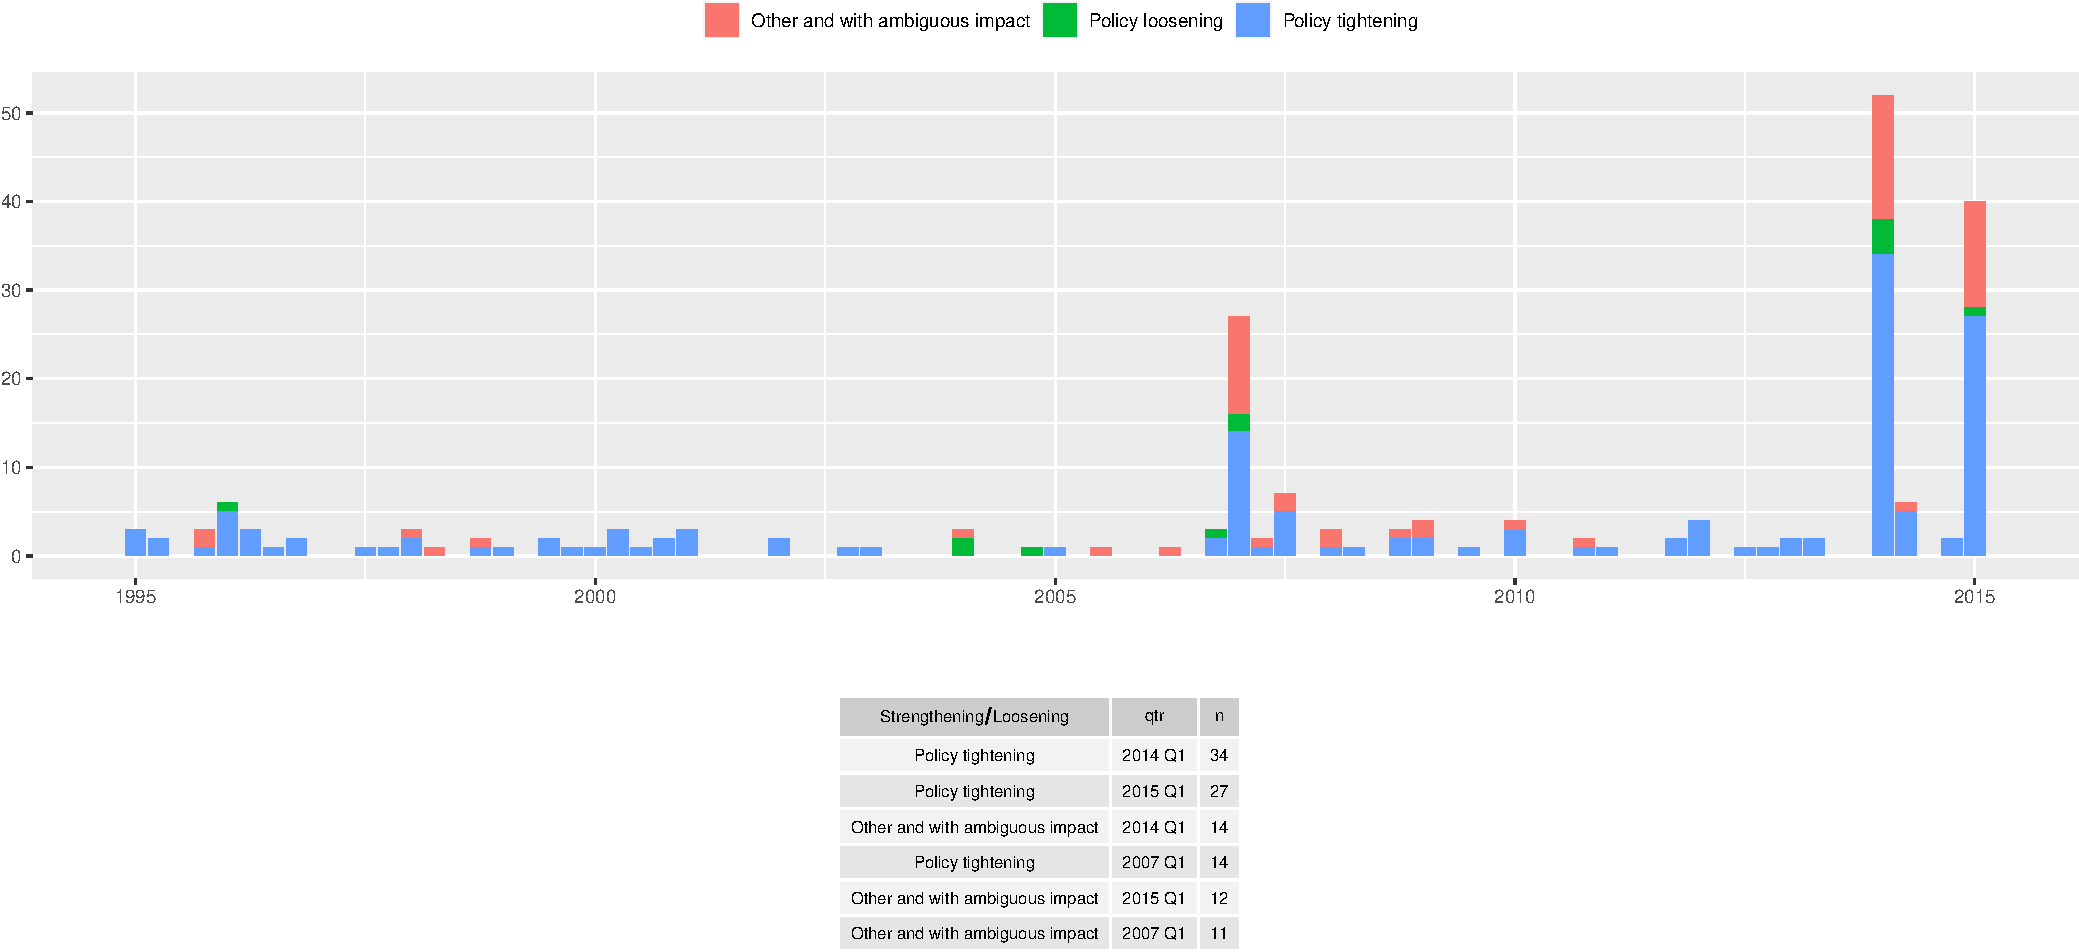
\includegraphics{figures/paper-fig1-1} \caption{Count of minimum capital requirements policy actions}\label{fig:fig1}
\end{figure}

Figure 1 describes the evolution of the MCR policy actions over the
sample period. The bottom panel indicates some spikes in activity,
notably in 2007 Q1, 2014 Q1, and 2015 Q1. These spikes are unsurprising
given the initial reactions to the crisis and the wave of regulatory
reform which swept through Europe in the subsequent period.

\hypertarget{meth}{%
\section{Methodology}\label{meth}}

We use a Bayesian inference framework to estimate systemic risk and
investigate the impact of policy actions. In a dynamic setting, this
offers some benefits compared to classical panel estimators. In contrast
to traditional approaches, which treat group-levels parameters as
nuisance parameter to be removed, Bayesian method provide explict
estimates of group-level parameters which can be regularised to include
only information that adds explanatory power. In the context of our
study, Bayesian methods can control for attenuation bias\footnote{Following
  Strauss and Yang (2020), we explicitly model measurement error using
  latent variables.} that is known to be associated with policy action
count data Akinci and Olmstead-Rumsey (2017). Finally, we include a
noise component to numerate the fluctuations in the panel structure of
the data.

\hypertarget{systemic-risk-measurement}{%
\subsection{Systemic risk measurement}\label{systemic-risk-measurement}}

We use the \(\Delta CoVaR\) approach to systemic risk estimation, which
extends the Value at Risk (VaR) concept to the system. \(CoVaR\) can be
thought of as the VaR of the whole system conditional on institution i
being in a certain state. Systemic risk is approximated using
\(\Delta CoVaR\); the difference between the \(CoVaR\) conditional on
the distress of an institution and the \(CoVaR\) conditional on the
median state of that institution. \(\Delta CoVaR\) is best thought of as
a reduced form statistical tool which captures tail codependency or the
part of systemic risk that co-moves with the distress of an institution.
\(\Delta CoVaR\) frames a bank as a \emph{risk inducer}, quantifying the
contribution of a financial institution to the system-level risk. This
is achieved by estimating the additional value at risk of the entire
financial system associated with this institution experiencing distress
(Brunnermeier, Rother, and Schnabel 2020).

Formally, Let \((Y_1,\dots,Y_d)\) be a d-dimensional random vector where
each \(Y_j\) is expressed through some covariates
\(X= (X_1,X_2,...,X_M)\). In the systemic risk context, \(Y_j\) denotes
the behaviour of either an institutions or the whole system. Without
loss of generality, thereafter, we fix \(\tau \in (0,1)\) and suppose
that we are interested in institutions j within system k. The
Value-at-Risk, \(VaR^{\bf{X},\tau}_j\) of institution j is the
\(\tau\)-th level conditional quantile of the random variable
\(Y_j|\bf{X}=x\):

\begin{equation}\label{eq:eq1}
\mathbb{P}(Y_j \leq VaR^{\bf{X},\tau}_j |\bf{X}=x)=\tau
\end{equation}

.The Conditional Value-at-Risk
\(\left( CoVaR_{system=k|j}^{\bf{X},\tau} \right)\)is the Value-at-Risk
of system k conditional on \(Y_j= VaR_j^{\bf{X}\tau}\) at the level
\(\tau\) which satisfies:

\begin{equation}\label{eq:eq2}
\mathbb{P}\left(Y_{system=k} \leq CoVaR_{system=k|j}^{\bf{X},\tau} |\bf{X}=x,Y_j=VaR^{\bf{X},\tau}_j \right)=\tau
\end{equation}

Using Bayesian inference, equation \ref{eq:eq2} implies that CoVaR
corresponds to the \(\tau\)-th percentile of the conditional
distribution (For a detailed exposition see Bernardi, Gayraud, and
Petrella 2013)

\hypertarget{bayesian-regularised-time-varying-delta-covar-estimation}{%
\subsection{\texorpdfstring{Bayesian regularised time-varying
\(\Delta CoVaR\)
estimation}{Bayesian regularised time-varying \textbackslash Delta CoVaR estimation}}\label{bayesian-regularised-time-varying-delta-covar-estimation}}

To capture all forms of risk including volatility feedback, adverse
asset price movements and funding liquidity risk, we estimate
\(\Delta CoVaR\) using daily return losses from 1995:I to 2018:IV for a
sample of European commercial banks, investment banks, insurance
companies and real estate companies. Return losses \(Y_{it}\) are
measured using market equity \(ME\) of the publicly traded institution,

\begin{equation}\label{eq:eq3}
Y_{i,t+1}=-log(ME_{i,t+1}/ME_{i,t})
\end{equation}

We extend the work of Bernardi, Gayraud, and Petrella (2013) by using an
Bayesian adaptive LASSO quantile regression to evaluate daily time
varying \(\Delta CoVaR\). Regularisation techniques, such as the LASSO,
have been shown to improve predictive accuracy of quantile regression by
only include information which adds to the predictive power of the
explanatory variable set (Li, Xi, and Lin 2010). Regularisation
techniques employed with Bayesian inference are increasing common in
financial econometric (See for example Tibshirani 2011; Mogliani and
Simoni 2020; Fan, Ke, and Wang 2020). The adaptive LASSO is especially
useful when estimated time-varying \(\Delta CoVaR\), given the noisy
nature of the macroeconomic variables used as state dynamics adjustors
(See Table A.1 for full list). Finally, in the context of systemic risk,
Bayesian methods are highly flexible and are extreme useful in the
context of the analysis of interdependence effects of extreme market
events. Using data and prior information they provide the complete
posterior distribution of the parameters of interest. Since the
quantities of interest in this paper are risk measures, learning about
the whole distribution becomes more relevant due to the interpretation
of \(CoVaR\) as financial losses (Bernardi, Gayraud, and Petrella 2013)

Formally, the Bayesian Adaptive Lasso regression is a hierarchical model
which exploits a skewed Laplace distribution\footnote{which has the
  attractive property of being represented as a scale mixture of normal
  distributions (Tsionas 2003)} to estimated \(VaR^{\bf{X},\tau}_j\) and
\(\left( CoVaR_{system=k|j}^{\bf{X},\tau} \right)\) as follows:

\begin{equation}\label{eq:eq4}
Y_{jt}=\beta_{0,j}+\bf{M^{'}_{i,t-1}} \bf{\beta_j} +\theta_j z_j+\phi \xi_j \sqrt{\sigma^{-1}z_j} 
\end{equation}

\begin{equation}\label{eq:eq5}
Y_{kt}=\beta_{0k}+\bf{M^{'}_{i,t-1}} \bf{\beta_k} +\delta Y_{jt}+\theta z_j+\phi\xi_k\sqrt{\sigma^{-1}z_k}
\end{equation}

where \(M\) is a set of European financial and macroeconomic variables
detailed in Table A.1 in the appendix.

\hypertarget{var-and-covar-posterior-estimation}{%
\subsubsection{VaR and CoVaR posterior
estimation}\label{var-and-covar-posterior-estimation}}

Our study captures an intuitively appealing complete probability
distribution of the phenomenon of interest\footnote{There is no free
  lunch, and bayesian inference comes at the cost of some additional
  assumptions, namely the setting of priors. That said, state-of-the-art
  bayesian inference provides tools to interrogated these assumptions
  using prior predictive checks. Given that Bayesian models are
  generative, prior predictive checks allow the use of a range of
  informative and non-informative priors to generate simulated data that
  can be checked against the actual data. This process is robust and is
  not subject to information leakage which can occur in classical model
  validation}. Conventionally, posterior probabilities using a maximum
of the posterior density (Maximum a Posteriori or \(MaP\))\footnote{MaPs
  are mathematically equivalent to the minimisation problem in the
  frequentist context (Lin and Chang 2012) and are equivalent to maximum
  likelihood estimates with flat priors} as a summary. We assume an
asymmetric Laplace distribution for the error terms and weakly
informative priors on the parameters\footnote{Prior predictive checks
  show that the size of the dataset quick dominants any undue influence
  of these priors and is available upon request from the author}. From
all the \(MaP\) parameters involved in the marginal and conditional
quantiles the estimates of \(VaR^{\bf{X},\tau}_j\) and
\(\left( CoVaR_{system=k|j}^{\bf{X},\tau} \right)\) are derived as
follows:

\begin{equation}\label{eq:eq6}
(VaR^{X,\tau}_j)^{MaP} = X^{'}\beta_j^{MaP}
\end{equation} \begin{equation}\label{eq:eq7}
(CoVaR_{system=k|j}^{X^{'},\tau})^{MaP} = X^{'} \beta_{system=k}^{MaP}+\delta^{MaP}(VaR^{\bf{X},\tau}_j)^{MaP}
\end{equation}

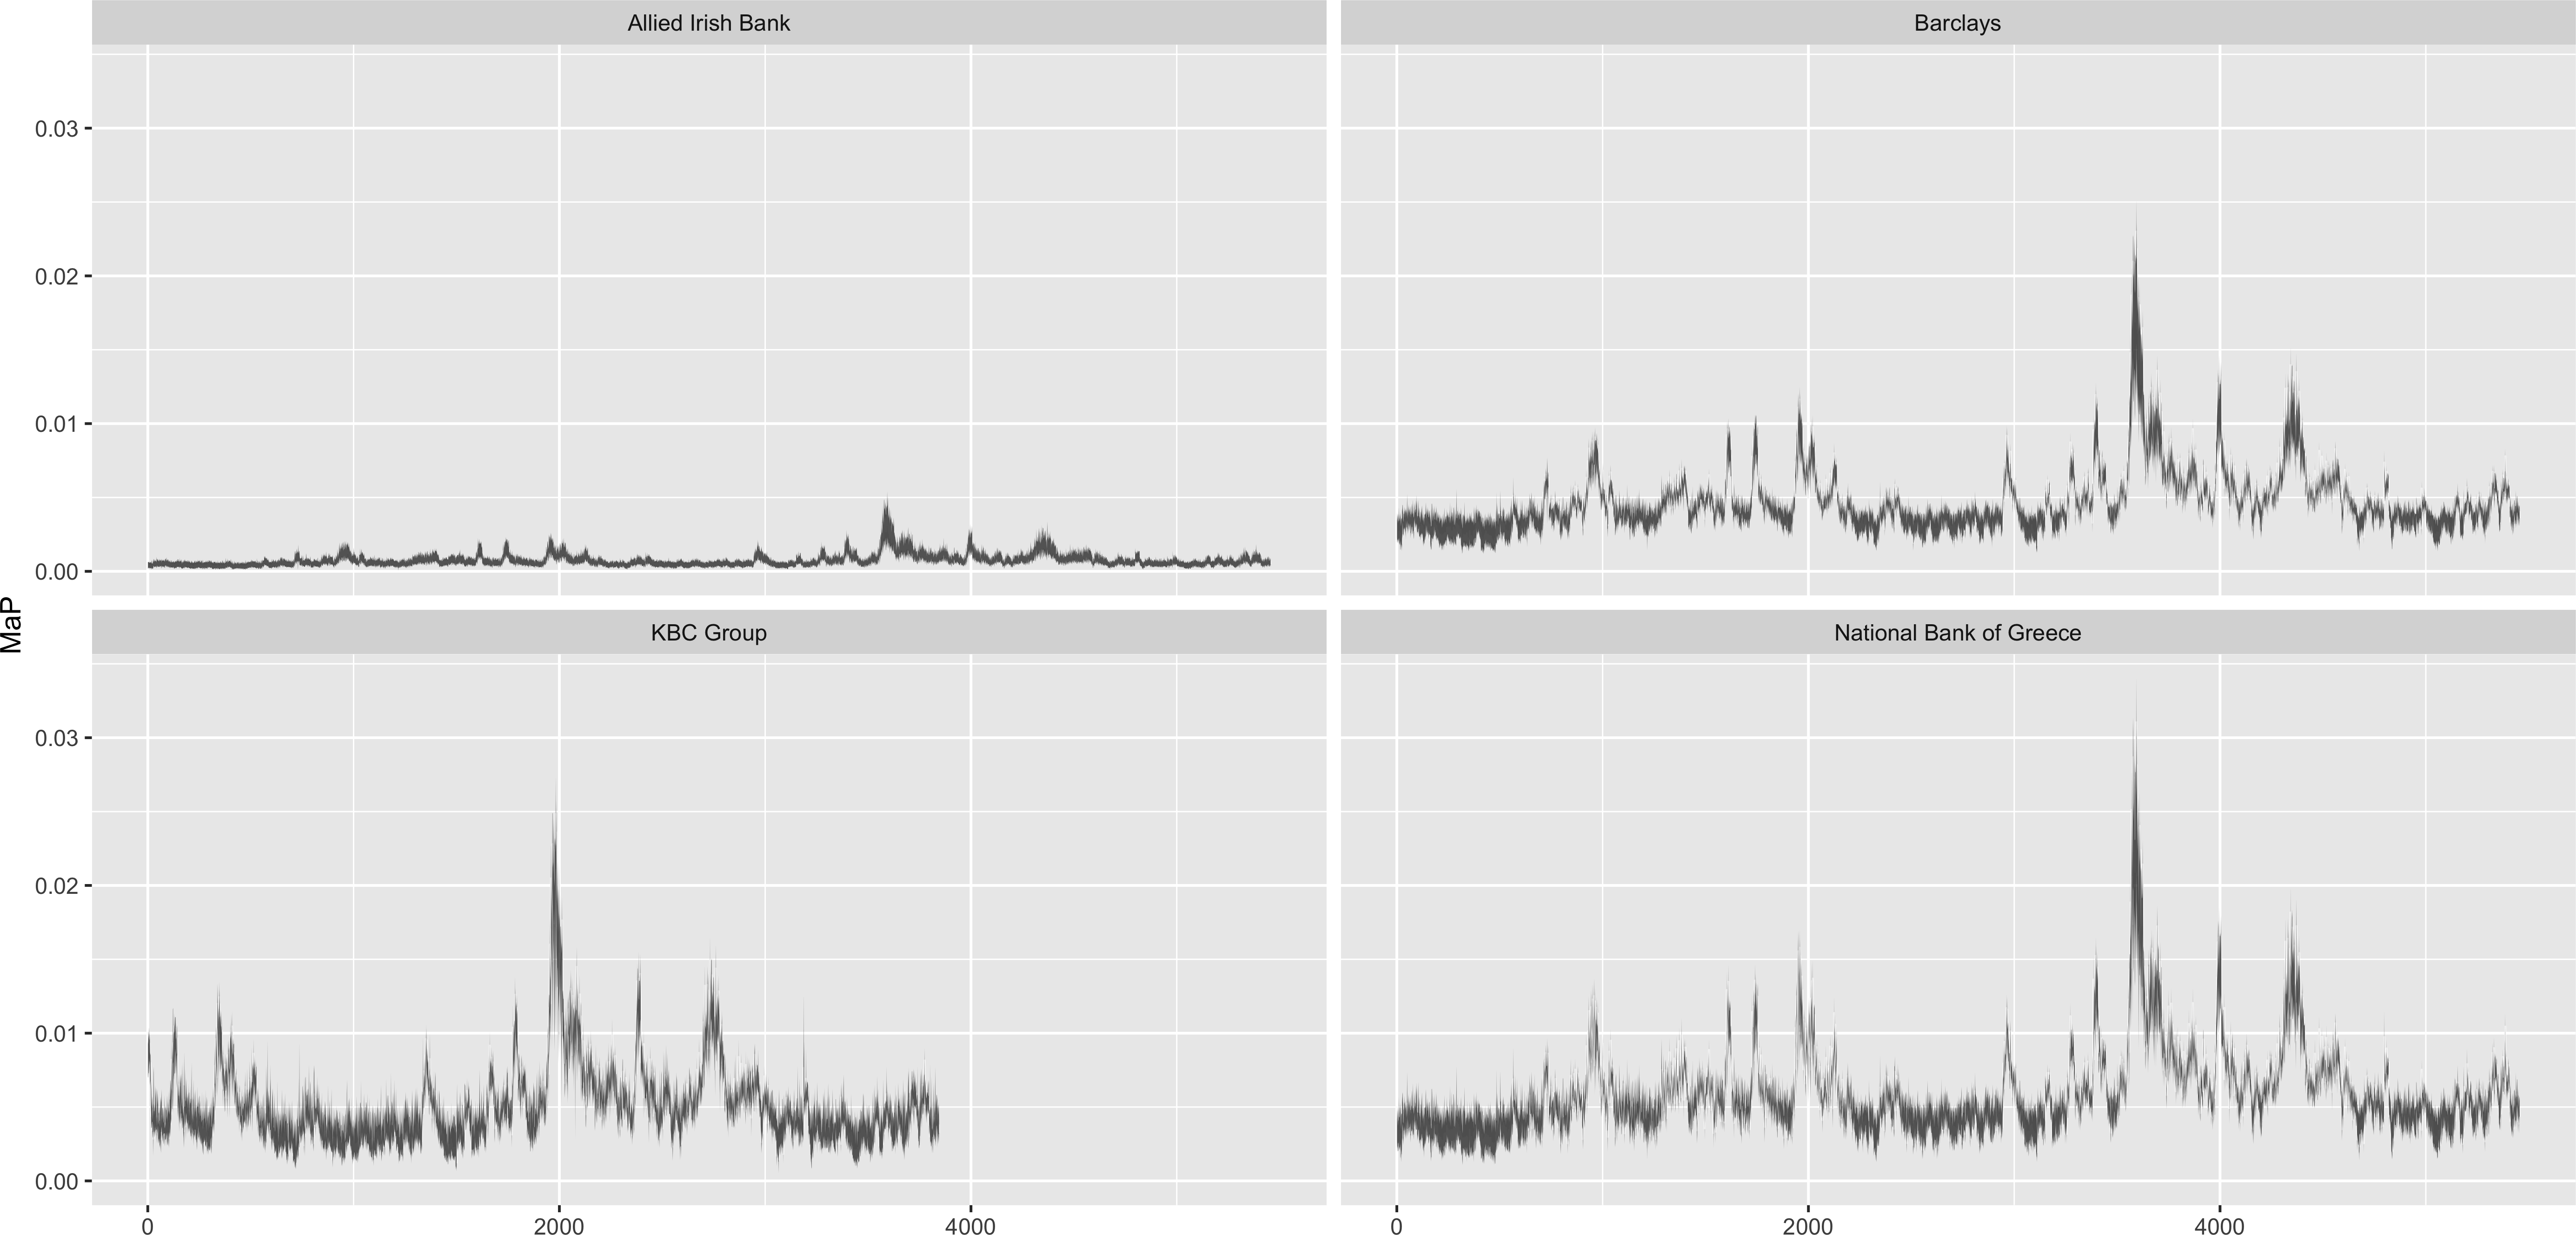
\includegraphics{figures/paper-build graphs-1}

Figure 2 visualised the \(\Delta CoVaR\) estimate for a small selection
of banks. In each plot the 99\% credibility set is represented by the
shaded area depicting the uncertainty in the MaP estimate. The x-axis is
a daily time indicator for the sample period. While the time patterns
are similar in each plot with a spike at the height of the European
crisis, KBC group, Barclays and National Bank of Greece stand out for
their significantly higher systemic risk inducing behaviour.

\hypertarget{bayesian-hierarchical-model}{%
\subsection{Bayesian Hierarchical
Model}\label{bayesian-hierarchical-model}}

This section will lay out the Bayesian hierarchical model used to the
effect of capital actions on systemic risk. Bayesian hierarchical or
multilevel models exploit a data structure with several levels that are
either nested or non-nested. The key to identifying a variable as a
level is that its units are a random sample from a wider population. In
this instance, we have a three-level nested data structure of repeat
observations within banks within European countries. The banks are a
random sample from a broader population of banks; likewise, the
countries are a random sample from many countries. In general,
multilevel models are helpful where relationships vary across
higher-level units\footnote{As a rule of thumb, the highest level should
  have at least 20 units to be suitable for this type of analysis
  (\url{http://www.bristol.ac.uk/cmm/learning/multilevel-models/data-structures.html})}.
This is in stark contrast to classical least squares regression models
where group effects are typically binary indicators, so-called
\emph{unit fixed effects} models (Imai and Kim 2019). Typically, a
\emph{fixed effects} model cannot discriminate between observed and
unobserved group characteristic effects (for example, a policy action
applied by the national regulator).\footnote{Econometrically, there is a
  confounding effect of the group level dummies on the group-level
  predictors.} What results from a fixed effect model is, at best, a
partial estimate of the ground truth. To date, there are a few notable
exceptions in panel data econometrics(see, for example, Wooldridge
(2019) correlated random effects model). There is no such issue with a
multilevel model, where full effects at many levels can be
simultaneously estimated.

\hypertarget{multilevels-delta-covar-regressions}{%
\subsubsection{\texorpdfstring{Multilevels \(\Delta CoVaR\)
Regressions}{Multilevels \textbackslash Delta CoVaR Regressions}}\label{multilevels-delta-covar-regressions}}

The regression models use MaP estimates of \(\Delta CoVaR\) for the 116
commercial banks as the dependent variable. Our hierarchical regression
model aims to extract meaningful effects of country-level policy actions
on bank-level systemic risk. Our strategy allows for (bank-level)
coefficients on the policy action variables to vary by country and
quarter, in addition to being `fixed'. We can think of these then as our
three \emph{random effects}. Denoting \(y_{c,t[i]}\) as the
\(\widehat{CoVaR_{c,t[i]}}\) estimate of firm \(i\) in-country in time
t, we set up two specifications. A baseline where we assume that policy
action effect across countries is constant. Then we relax this
assumption allowing banks in each country to experience their effect,
which is then regularised, via partial pooling towards a global mean.
Equation \ref{eq:eq8} describes our baseline model (regression 1), while
\ref{eq:eq9} describes the more flexible country-level \emph{random
effects} model (regression 2).

\begin{equation}\label{eq:eq8}
 y_{c,t[i]} = (\alpha + \alpha_{c,t}) + \beta^L loose_{c,t}+\beta^T tight_{c,t}+\beta^A ambig_{c,t}+Bank_Adjustments_{c,t[i]}+M_{c,t}+\epsilon_{c,t[i]}
\end{equation}

\begin{equation}\label{eq:eq9}
y_{c,t[i]} = (\alpha + \alpha_{c,t}) + (\beta^L+\beta^L_{c,t})loose_{c,t}+(\beta^T+\beta^T_{c,t})tight_{c,t} \\
  +(\beta^A+\beta^A_{c,t})ambig_{c,t}++Bank_Adjustments_{c,t[i]}+M_{c,t}+\epsilon
\end{equation}

\(\alpha, \beta^L, \beta^T\) and \(\beta_A\) are the \emph{fixed} effect
population coefficients that represent the global \emph{average}
intercept and globe slope coefficients our policy actions variables for
a total pooled sample. \(\beta^L_{c,t},\beta^T_{c,t},\beta^A_{c,t}\) are
the \emph{random} effects counterparts and represent the slope
coefficients for each of the 22 countries \(c\) and 83 quarters \(t\).
The \emph{random} policy effect coefficient estimates, for each country
or year, deviates from the population average; such that
\(\beta^T_{c,t}\) describes how the systemic risk impact of tightening
policy actions in the country \(c\) or year \(t\) deviates from the
average impact across all countries and quarters.

Following Brunnermeier, Rother, and Schnabel (2020), we use a concise
set of bank-level and macro-level adjustments\footnote{The common
  practice use of \emph{control} when describing the adjudicating
  variables in a regression implies overconfidence in the analyst's
  ability and is sloppy statistical language. The true meaning of a
  \emph{control} variables is when we can intervene and change the
  variable by a certain amount, which is clearly not possible in any
  observational studies. We, therefore, prefer the more modest and
  realistic \emph{adjusting} description}. The bank-level variables
include (i) leverage, measured as the ratio of total assets to common
equity; (ii) maturity mismatch, measured as short-term borrowings to
total assets; (iii) size, measured as the log of market equity, (iv)
loan growth measures as the percentage change in gross loans, and (v) an
asset price boom indicator, which is the number of consecutive quarters
of being in the top decile of the price to book ratio across all firms.
The macro-level variable set \(M\) is the same as that used in the
time-varying systemic risk estimation. Finally, we include an AR(1)
error process to adjust for the panel nature of our data, which are
excluded from the already crowded specification above.

\hypertarget{robustness-and-endogeniety}{%
\subsection{Robustness and
Endogeniety}\label{robustness-and-endogeniety}}

We undertake a barrage of test and alternative specifications. By its
theoretical nature systemic risk, and its joint distribution with policy
actions is a rare event phenomenon. Capturing this feature in the
conditional distribution of our hierarchical regression may require more
nuanced distributional assumptions than normality. To this end, we
consider three alternative probability distributions, skewed-normal,
t-distribution and log-normal. Widely Accepted Information Criteria
(WAIC) suggest that the t-distribution is the most appropriate among
these alternatives, which conforms with expert advice when modelling
extreme events in hierarchical models (Gelman et al. 2019). The reported
results are those based on a t-distribution. Heteroskedasticity is model
explicitly through our varying-coefficients approach, with each group in
our model having its variance parameter, in addition to the pooled
(country-level) error (Sims 2010). We interrogate different priors,
which have almost no impact on our coefficient estimates. These results
are unsurprising given that a large amount of data will usually render
redundant the influence of priors. We have explored different random
effect coefficients based on different clusterings in the data, by bank
size, at the bank level. The resultant variation cuts across clusters
and obfuscates the phenomenon of interest. Finally, when we remove the
country and year group from the random effects, then the variation in
the data is misappropriated to a different \emph{level}(Schmidt-Catran
and Fairbrother 2015).

Endogeneity is a common challenge when investigating the risk
implications of regulatory actions (See Appendix for a theoretical
treatment of over policy actions treatment). For example, naturally
clustered data typically exhibits a correlation of unobserved shocks
within a country, a quarter or a quarter specific quarter within a
country (Wooldridge 2010).In our model, this correlation is model
directly. More precisely, the model includes one error term attributed
to all banks within each group of the model (plus the pooled regression
level error). These terms capture correlation across banks; within the
same quarter, within the same country, and the same quarter for a
country. Put differently, our model best deals with unobserved
heterogeneity by directly modelling it by allowing slopes and intercepts
to vary across country and year clusters. Ignoring parameter
heterogeneities among cross-sectional or time-varying units can lead to
non-sensical parameter estimates if the average has no
representativeness across individual countries or quarters, in our case
(Hsiao 2014).

Endogeneity is a particular concern in firm-level regression for several
reasons -- especially when the dependent variable is systemic risk. For
one, right-hand side variables in such regressions are invariably
endogenous, and an intractable identification problem arises due to the
simultaneity present. Adding lagged dependant variables does nothing to
deal with simultaneity bias, contrary to conventional belief(Reed 2015).
However, lagging the dependant variable has significant data
requirements. It introduces other forms of survivor bias, excluding
firms who do not conform to the balance panel (such as newer established
firms). Instead, we include a lagged AR(1) error structure to deal with
serial correlation and the dynamic structure of the model. This
autoregression term is measured precisely in our model, with a 95\%
credible interval {[}0.47,0.54{]}\footnote{Adding a second
  autoregressive error does not improve model fit much, has a small
  coefficient, and adds significant computational time}.

Secondly, endogeneity in regulation-systemic risk regressions is endemic
if regulation is mismeasured (Akinci and Olmstead-Rumsey 2017). In such
cases, a policy action count might not fully capture banks' future
systemic risk sensitivity due to the non-linear cumulative effect of
multiple policy actions. Measurement error in each policy action count
not only biases downward their specific coefficients but also
complicates the other actions' sensitivity interpretations. For
instances, if the \emph{tight} variable is measured with error due to a
count underestimating the causal mechanism of tightening policy actions
and the average \emph{tight} attenuates from the marginal \emph{tight}.
Measurement error is \emph{tight} not only biases the \emph{tight}
coefficients downwards but complicates the interpretation of
\emph{loose} to measure systemic risk sensitivity. It follows that
mismeasurement of \emph{tight}, could result in \emph{loose} impacting
systemic risk only because it is correlated with the \emph{ground truth}
(perfectly measured) marginal \emph{tight} which acts on banks' to
reduce their systemic risk inducing behaviour. Therefore, correcting for
mismeasurement error in each of our policy actions sum variables is
vital for proper inference from the others.

Care must be taken in what estimator to use in the context of
measurement error. Some commonly used estimators, such as first
differencing, will increase the bias size (Wooldridge 2015). On the
other hand, a Bayesian approach to measurement error is computationally
demanding but has several advantages. Firstly, the Bayesian estimator
provides a posterior distribution that accounts for parameter
uncertainty. In contrast, the classical estimator corrected for
attenuation would require bootstrapping or some asymptotic approximation
to account for this uncertainty---secondly, Bayesian inference averages
over plausible values of mismeasured policy actions in light of the
data. In contrast, traditional approaches impute a single best guess and
then proceeding as if this guess is correct. Policy actions casual
impact are capture with model uncertainty embedded. Thirdly, we can
integrate the measurement error with a more complex model: essentially
keeping our random effects structure, an autoregressive error structure,
a student-t likelihood, and other deviations from a simplistic panel
regression model (Carroll et al. 2006). Finally, a Bayesian approach to
measurement error encodes the \emph{true} quantities of interest as
missing data (Gelman et al. 2013). The complete model is detailed are
available in Appendix.

\hypertarget{results}{%
\section{Results}\label{results}}

Table 3 and 4 present regression results for our baseline and multilevel
models. The baseline model assumes policy actions effects are constant
over time and across the country. Predictors are standardised. For
brevity, bank-level parameter posterior probabilities are not shown in
the baseline model. In both instances, the Bayesian \(R^2\) indicates
the model \emph{fit}\footnote{We follow the procedure outline in Gelman
  et al. (2019), which calculates the Bayesian Bayesian \(R^2\) as the
  variance of the predicted values divided by the variance of the
  predicted values plus the expected variance of the errors} is very
good. For the baseline and multilevel model 95\% interval for the
Bayesian \(R^2\) are \([0.781,0,793]\) and \([0.885,0.891]\)
respectively. Both models allow the effects to be correlated, but
correlation coefficient estimates are not reported as they are not
significant. Robustness checks show that results are stable to the use
of different priors and likelihoods.\footnote{Fixed effect coefficients
  are almost identical, while there is some non-critical variation in
  the random effects occurs. The Bayesian \(R^2\) for the normal
  likelihood is smaller than the student-t by around 9\%-13\%}.

\begin{longtabu} to \linewidth {>{\centering}X>{\centering}X>{\centering}X>{\centering}X}
\caption{\label{tab:baseline}Summary of Baseline Model Regression Results}\\
\toprule
Variable & Estimate & l-95 CI & u-95 CI\\
\midrule
\addlinespace[0.3em]
\multicolumn{4}{l}{\textbf{Fixed Effects}}\\
\hspace{1em}\cellcolor{gray!6}{$\alpha$} & \cellcolor{gray!6}{12.851} & \cellcolor{gray!6}{8.949} & \cellcolor{gray!6}{16.932}\\
\hspace{1em}$\beta^A$ & 0.007 & -0.079 & 0.096\\
\hspace{1em}\cellcolor{gray!6}{$\beta^L$} & \cellcolor{gray!6}{-0.130} & \cellcolor{gray!6}{-0.399} & \cellcolor{gray!6}{0.143}\\
\hspace{1em}$\beta^T$ & 0.058 & 0.011 & 0.105\\
\addlinespace[0.3em]
\multicolumn{4}{l}{\textbf{Random Intercepts}}\\
\hspace{1em}\cellcolor{gray!6}{$\sigma_{\alpha_c}$} & \cellcolor{gray!6}{8.697} & \cellcolor{gray!6}{6.068} & \cellcolor{gray!6}{12.553}\\
\hspace{1em}$\sigma_{\alpha_t}$ & 0.904 & 0.765 & 1.074\\
\addlinespace[0.3em]
\multicolumn{4}{l}{\textbf{Student-t Parameters}}\\
\hspace{1em}\cellcolor{gray!6}{$\sigma$} & \cellcolor{gray!6}{0.707} & \cellcolor{gray!6}{0.692} & \cellcolor{gray!6}{0.722}\\
\hspace{1em}$\nu$ & 1.001 & 1.000 & 1.004\\
\bottomrule
\end{longtabu}

\begin{longtabu} to \linewidth {>{\raggedright}X>{\centering}X>{\centering}X>{\centering}X>{\centering}X>{\centering}X}
\caption{\label{tab:mixedeffects}Summary of Hierarchical Model Regression Results}\\
\toprule
  & Estimate & Est.Error & l-95 CI & u-95 CI & $R_hat$\\
\midrule
\addlinespace[0.3em]
\multicolumn{6}{l}{\textbf{Fixed Effects}}\\
\hspace{1em}\cellcolor{gray!6}{Intercept} & \cellcolor{gray!6}{13.146} & \cellcolor{gray!6}{2.005} & \cellcolor{gray!6}{9.154} & \cellcolor{gray!6}{17.214} & \cellcolor{gray!6}{1.005}\\
\hspace{1em}$B_{Size}$ & 0.114 & 0.012 & 0.031 & 0.164 & 1.000\\
\hspace{1em}\cellcolor{gray!6}{$B_{Leverage}$} & \cellcolor{gray!6}{0.511} & \cellcolor{gray!6}{0.112} & \cellcolor{gray!6}{0.110} & \cellcolor{gray!6}{0.810} & \cellcolor{gray!6}{1.000}\\
\hspace{1em}$B_{MaturityMismatch}$ & -0.221 & 0.012 & 0.201 & 0.251 & 1.000\\
\hspace{1em}\cellcolor{gray!6}{$B_{loanGrowth}$} & \cellcolor{gray!6}{0.012} & \cellcolor{gray!6}{0.005} & \cellcolor{gray!6}{0.000} & \cellcolor{gray!6}{0.002} & \cellcolor{gray!6}{1.000}\\
\hspace{1em}$B_{Boom}$ & 0.810 & 0.120 & 0.410 & 0.551 & 1.000\\
\addlinespace[0.3em]
\multicolumn{6}{l}{\textbf{Country Random Effects}}\\
\hspace{1em}\cellcolor{gray!6}{sd(Intercept)} & \cellcolor{gray!6}{8.687} & \cellcolor{gray!6}{1.620} & \cellcolor{gray!6}{6.006} & \cellcolor{gray!6}{12.325} & \cellcolor{gray!6}{1.015}\\
\hspace{1em}sd(tightSum) & 0.079 & 0.052 & 0.005 & 0.201 & 1.006\\
\hspace{1em}\cellcolor{gray!6}{sd(looseSum)} & \cellcolor{gray!6}{0.044} & \cellcolor{gray!6}{0.058} & \cellcolor{gray!6}{0.001} & \cellcolor{gray!6}{0.189} & \cellcolor{gray!6}{1.000}\\
\hspace{1em}sd(ambigSum) & 0.060 & 0.042 & 0.002 & 0.159 & 1.003\\
\addlinespace[0.3em]
\multicolumn{6}{l}{\textbf{Quarter Random Intercepts}}\\
\hspace{1em}\cellcolor{gray!6}{sd(Intercept)} & \cellcolor{gray!6}{0.912} & \cellcolor{gray!6}{0.084} & \cellcolor{gray!6}{0.767} & \cellcolor{gray!6}{1.094} & \cellcolor{gray!6}{1.001}\\
\addlinespace[0.3em]
\multicolumn{6}{l}{\textbf{Student-t Parameters}}\\
\hspace{1em}sigma & 0.707 & 0.008 & 0.692 & 0.722 & 1.003\\
\hspace{1em}\cellcolor{gray!6}{nu} & \cellcolor{gray!6}{1.001} & \cellcolor{gray!6}{0.001} & \cellcolor{gray!6}{1.000} & \cellcolor{gray!6}{1.004} & \cellcolor{gray!6}{1.000}\\
\bottomrule
\end{longtabu}

Several initial findings are noteworthy. There is a statistically
credible positive link between the build-up of tightening policy actions
and systemic risk one quarter on. Specifically our baseline model
estimates a global random effect of 0.058 with a 95\% posterior credible
interval of {[}0.011,0.105{]}. The estimates of equation \ref{eq:eq8}
provide a more complex set of outputs (this model has 473 parameters)
which are best-summarised visually\footnote{The direct frequentist
  counterpart to this model is a mixed effect model estimated by
  maximising a multivariate normal likelihood. Technically, these models
  treat group-level parameter estimates as a random variable that
  marginalises out to become part of the error term. Traditional
  ``fixed-effects'' panel data analytics perform a similar operation to
  remove group-level parameters. However, the group-level effects cannot
  be recovered, meaning the model coefficient represent a partial effect
  that ignores group-level covariance.}

\begin{figure}[H]
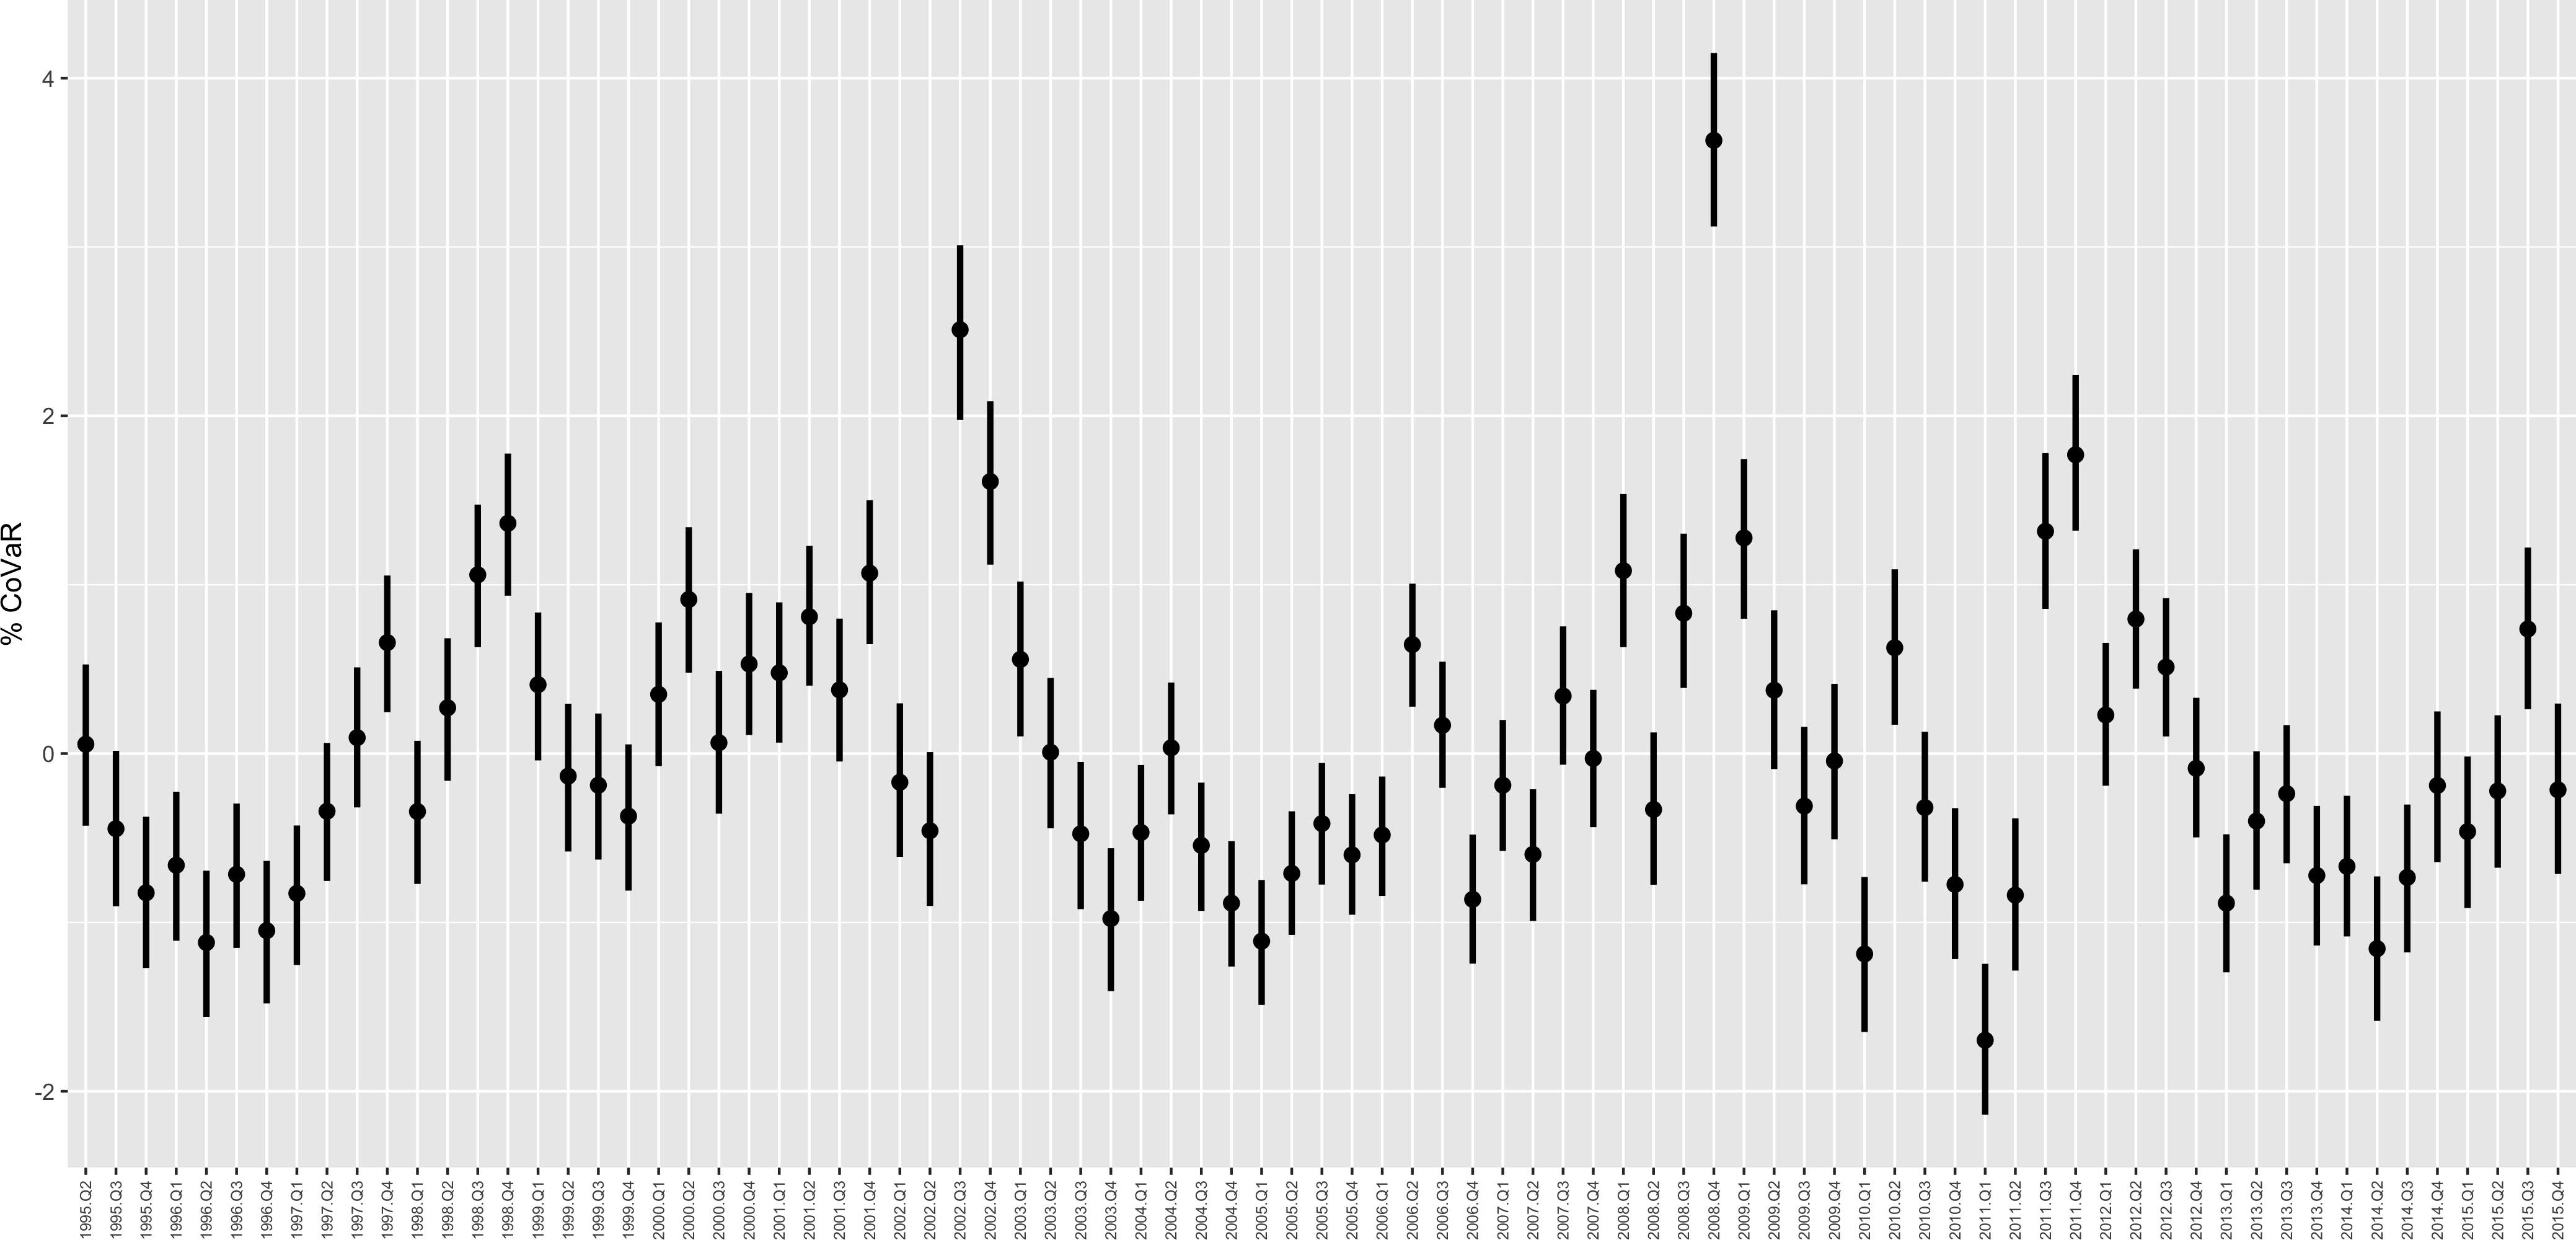
\includegraphics{figures/paper-fig3-1} \caption{Posterior probability distributions for quarter random intercepts}\label{fig:fig3}
\end{figure}

Figure 2 provides \emph{random} effects and their 99\% intervals for the
quarterly intercept parameters for the \(CoVaR^{99}_{it}\) regressions.
The estimate shows a clear risk pattern which peaks in 2008:Q4, the
epicentre of the recent financial crisis in Europe.

\begin{figure}[H]
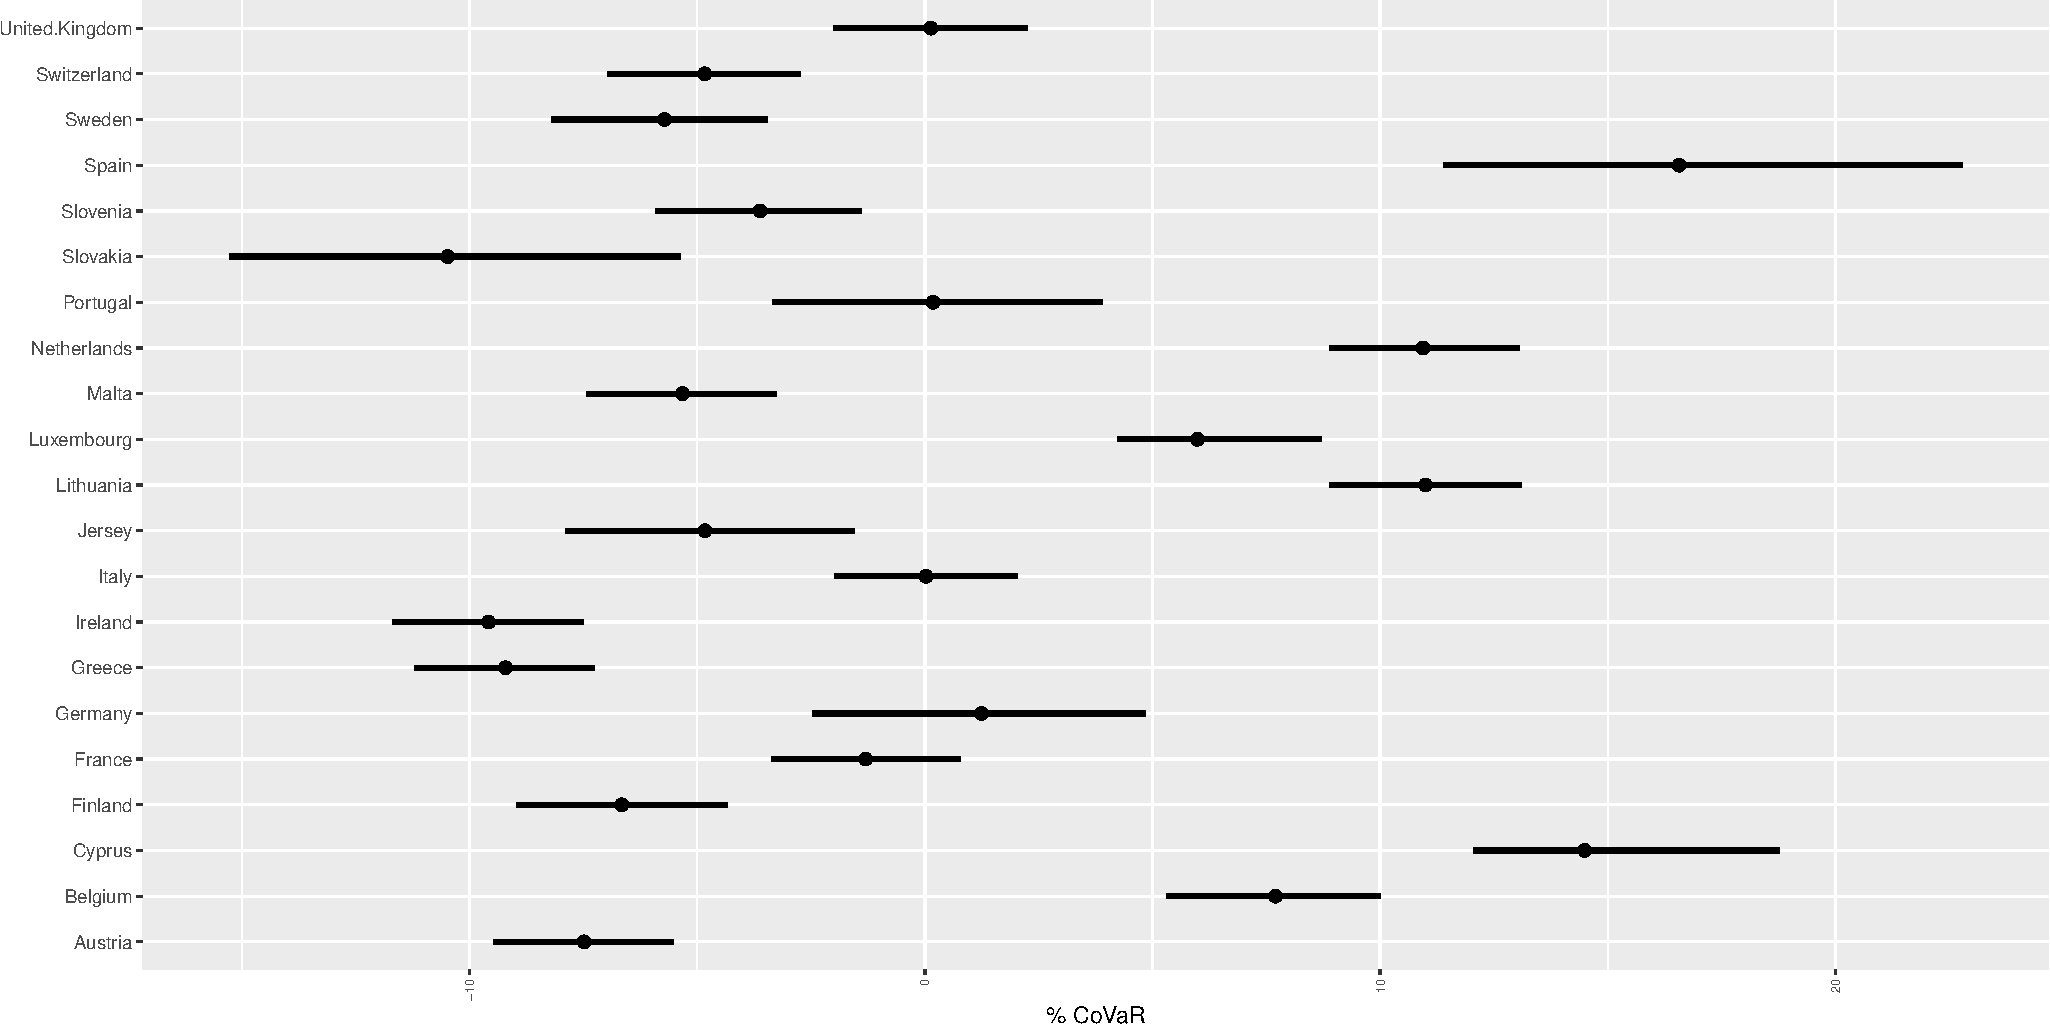
\includegraphics{figures/paper-fig4-1} \caption{Posterior probability distributions for country random intercepts}\label{fig:fig4}
\end{figure}

Figure 3 illustrates country-level random intercepts and show that banks
in each country are experiencing meaningful different systemic risk
contributions hold all else equal.

\begin{figure}[H]
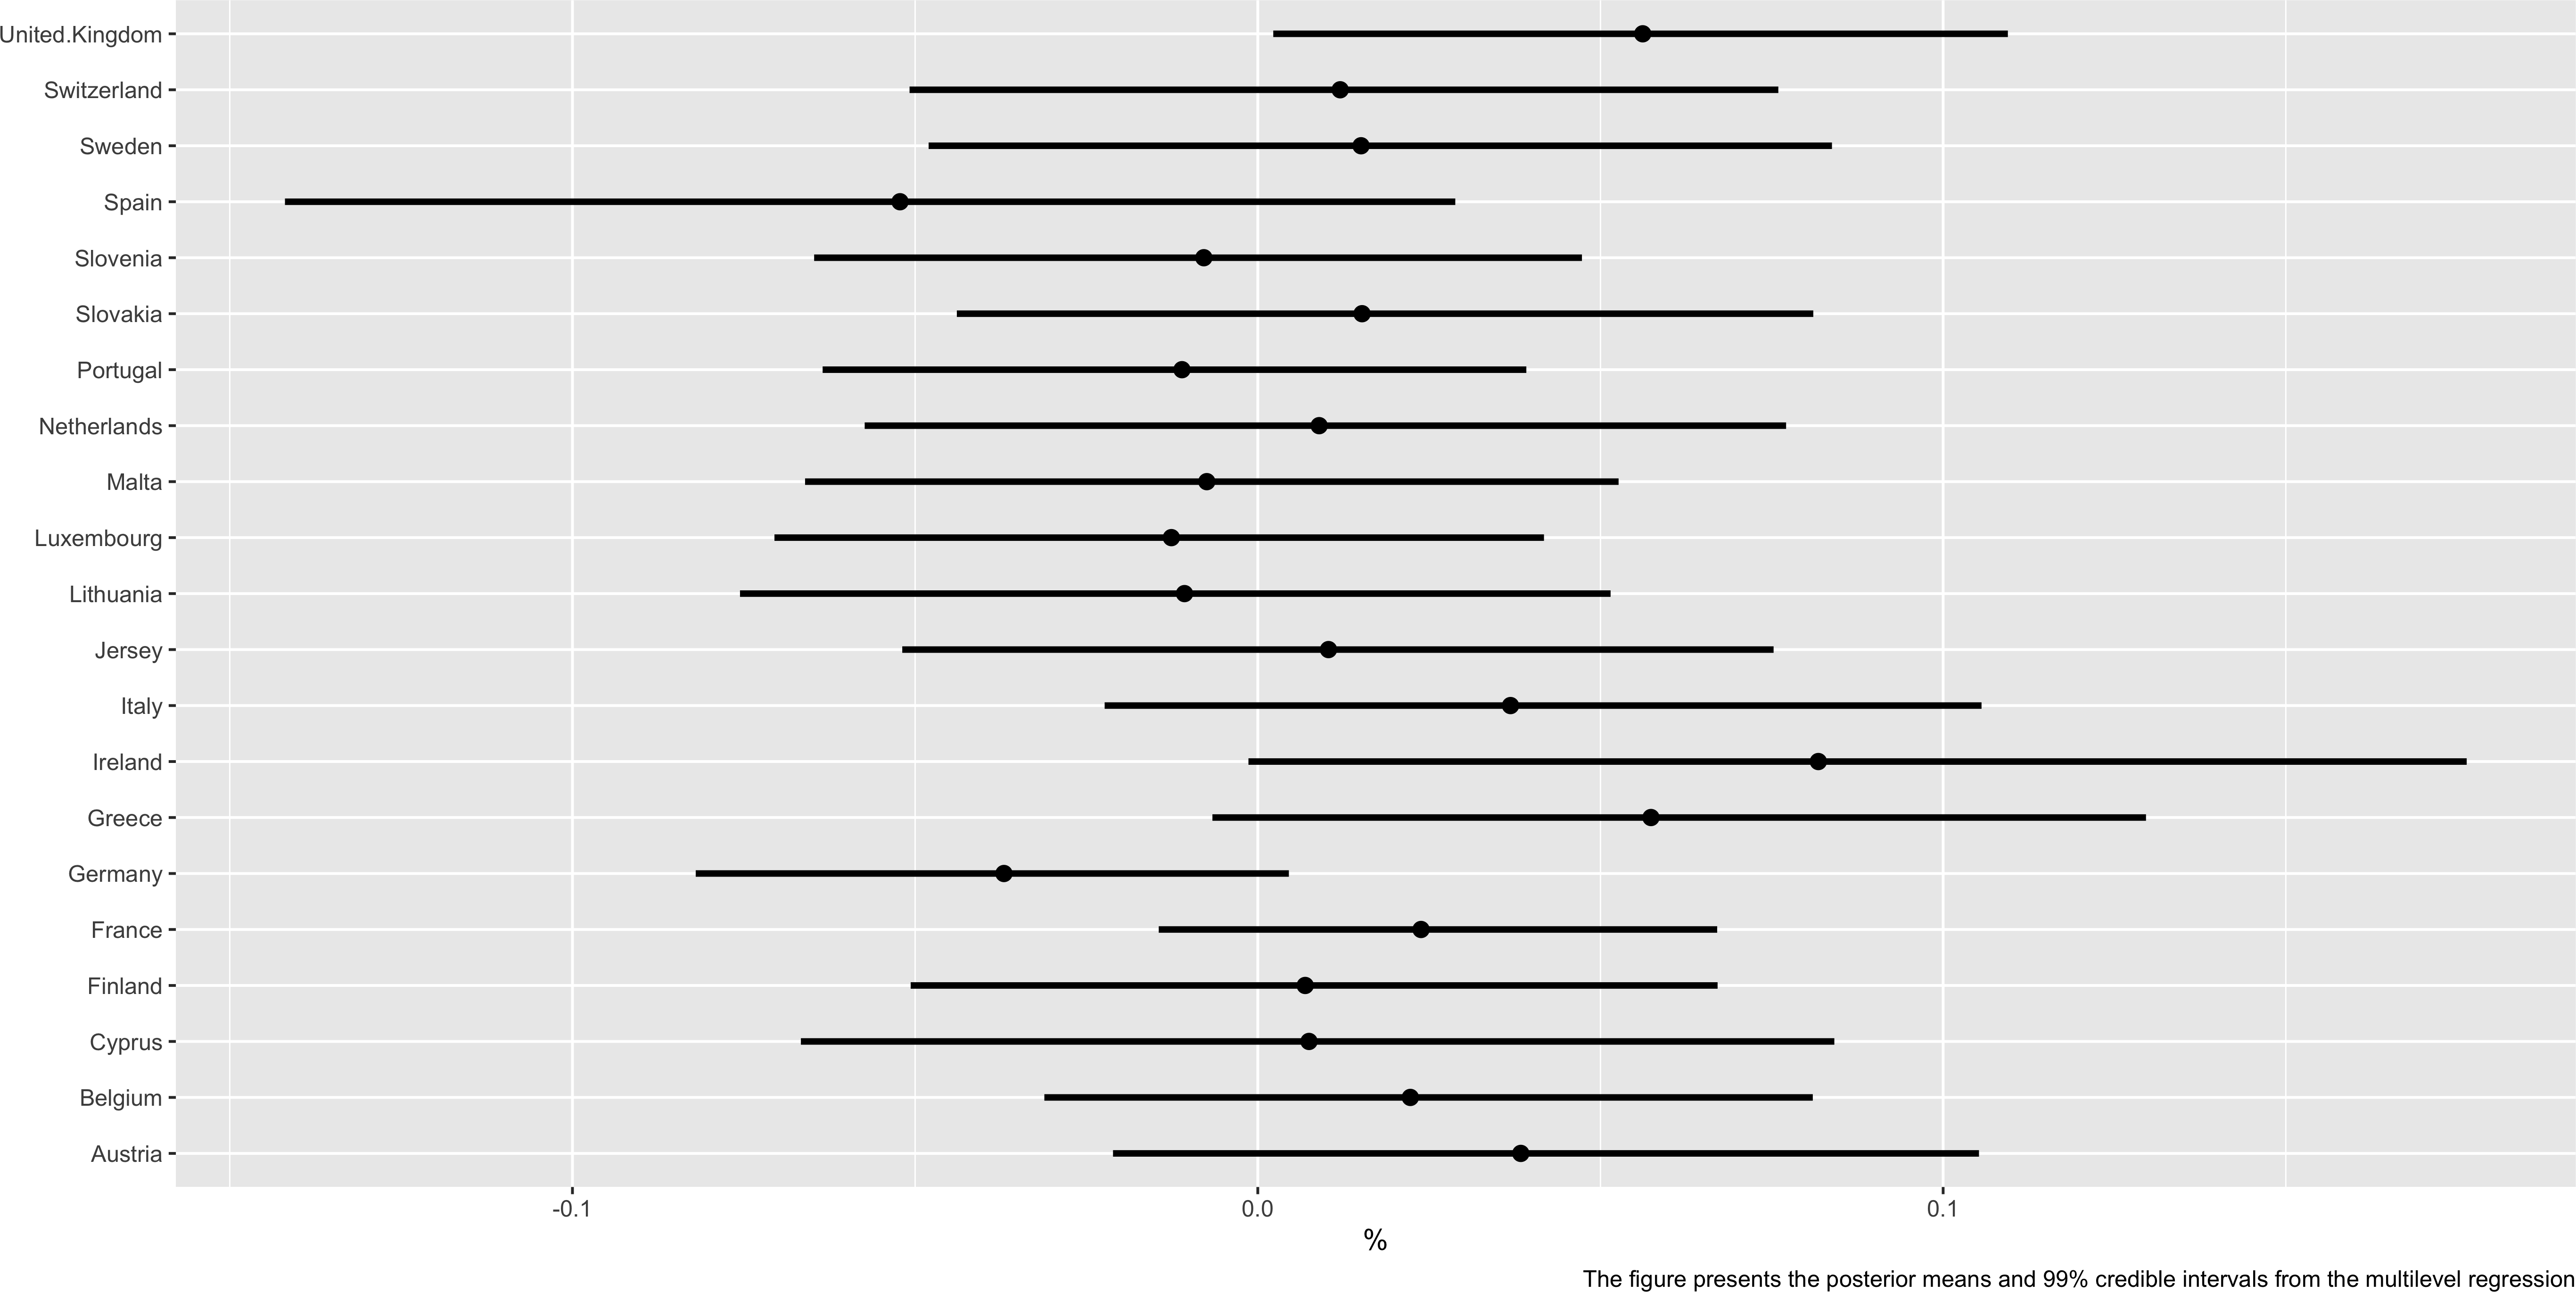
\includegraphics{figures/paper-fig5-1} \caption{Posterior probability distributions for country level random effects of tightening policy actions}\label{fig:fig5}
\end{figure}

\begin{figure}[H]
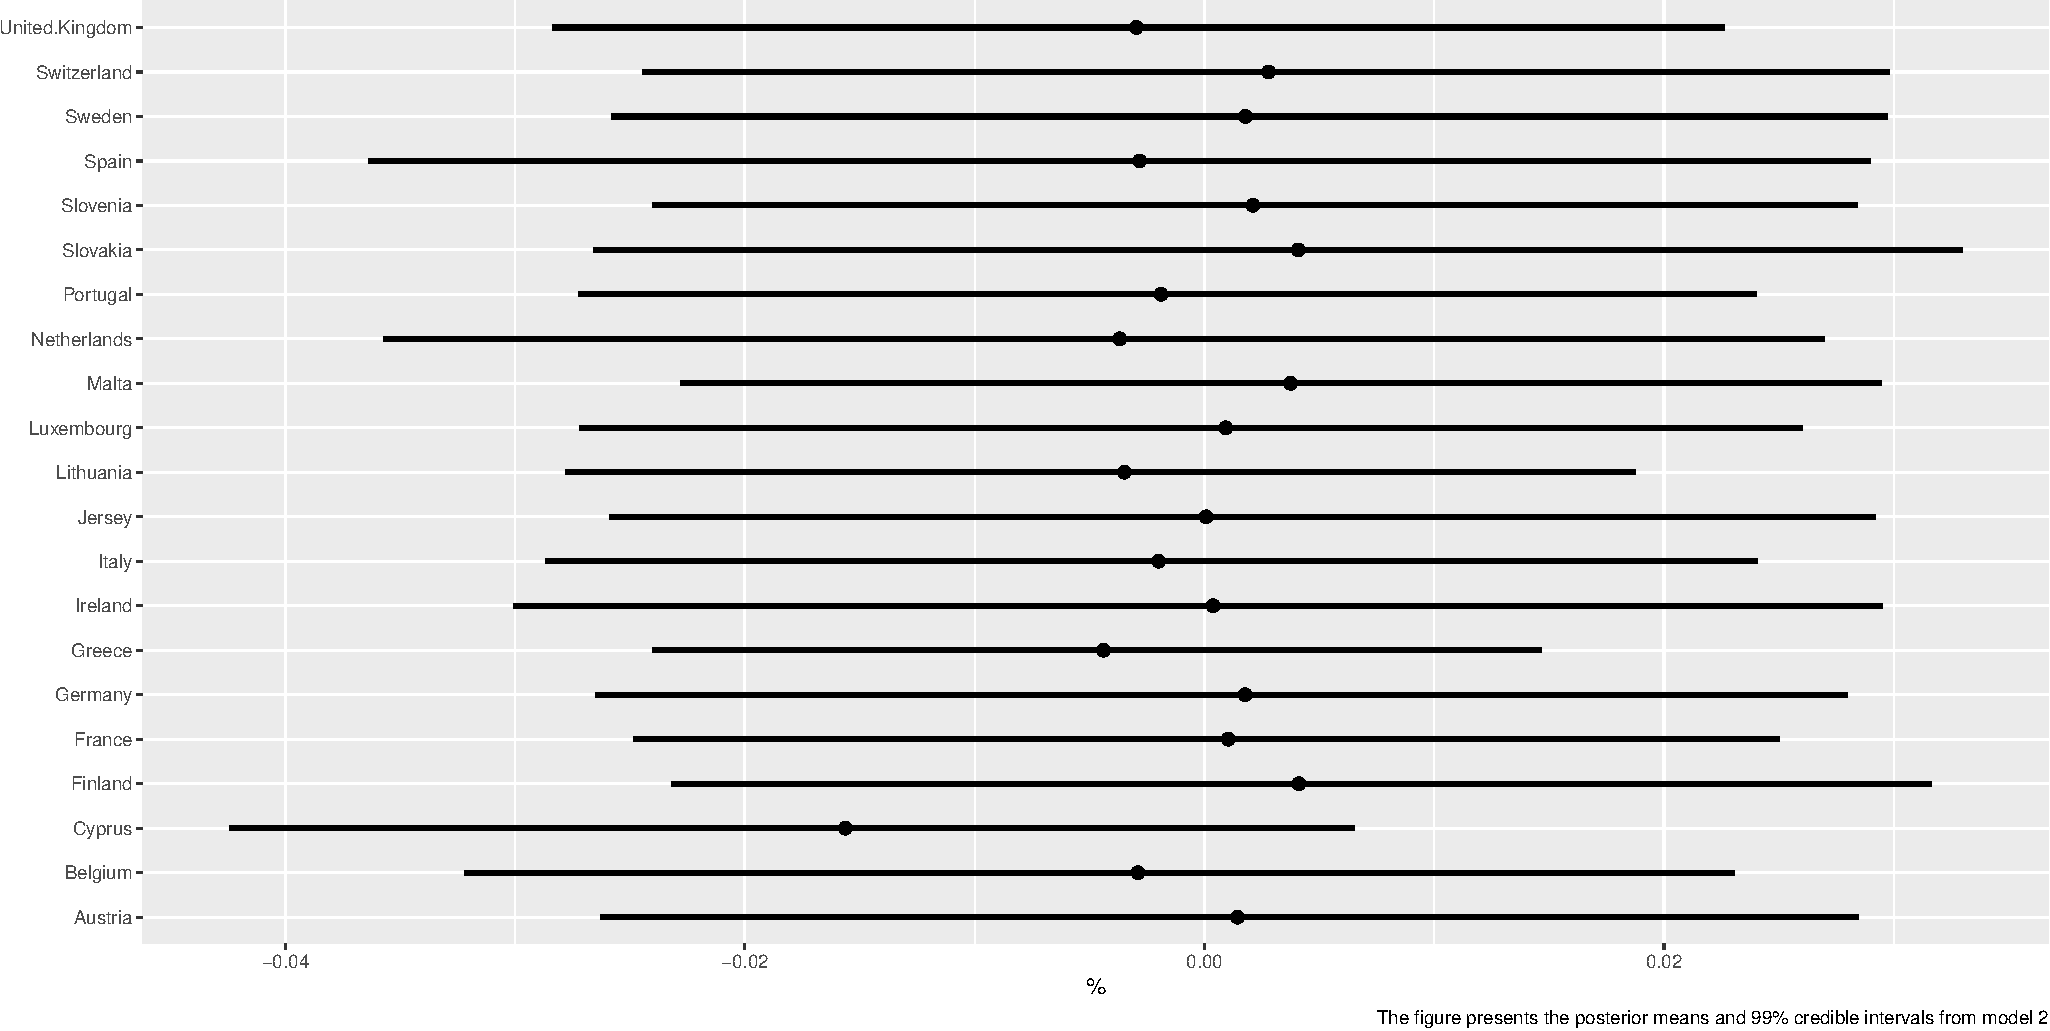
\includegraphics{figures/paper-fig6-1} \caption{Posterior probability distributions of country level random effects of loosening policy actions}\label{fig:fig6}
\end{figure}

\begin{figure}[H]
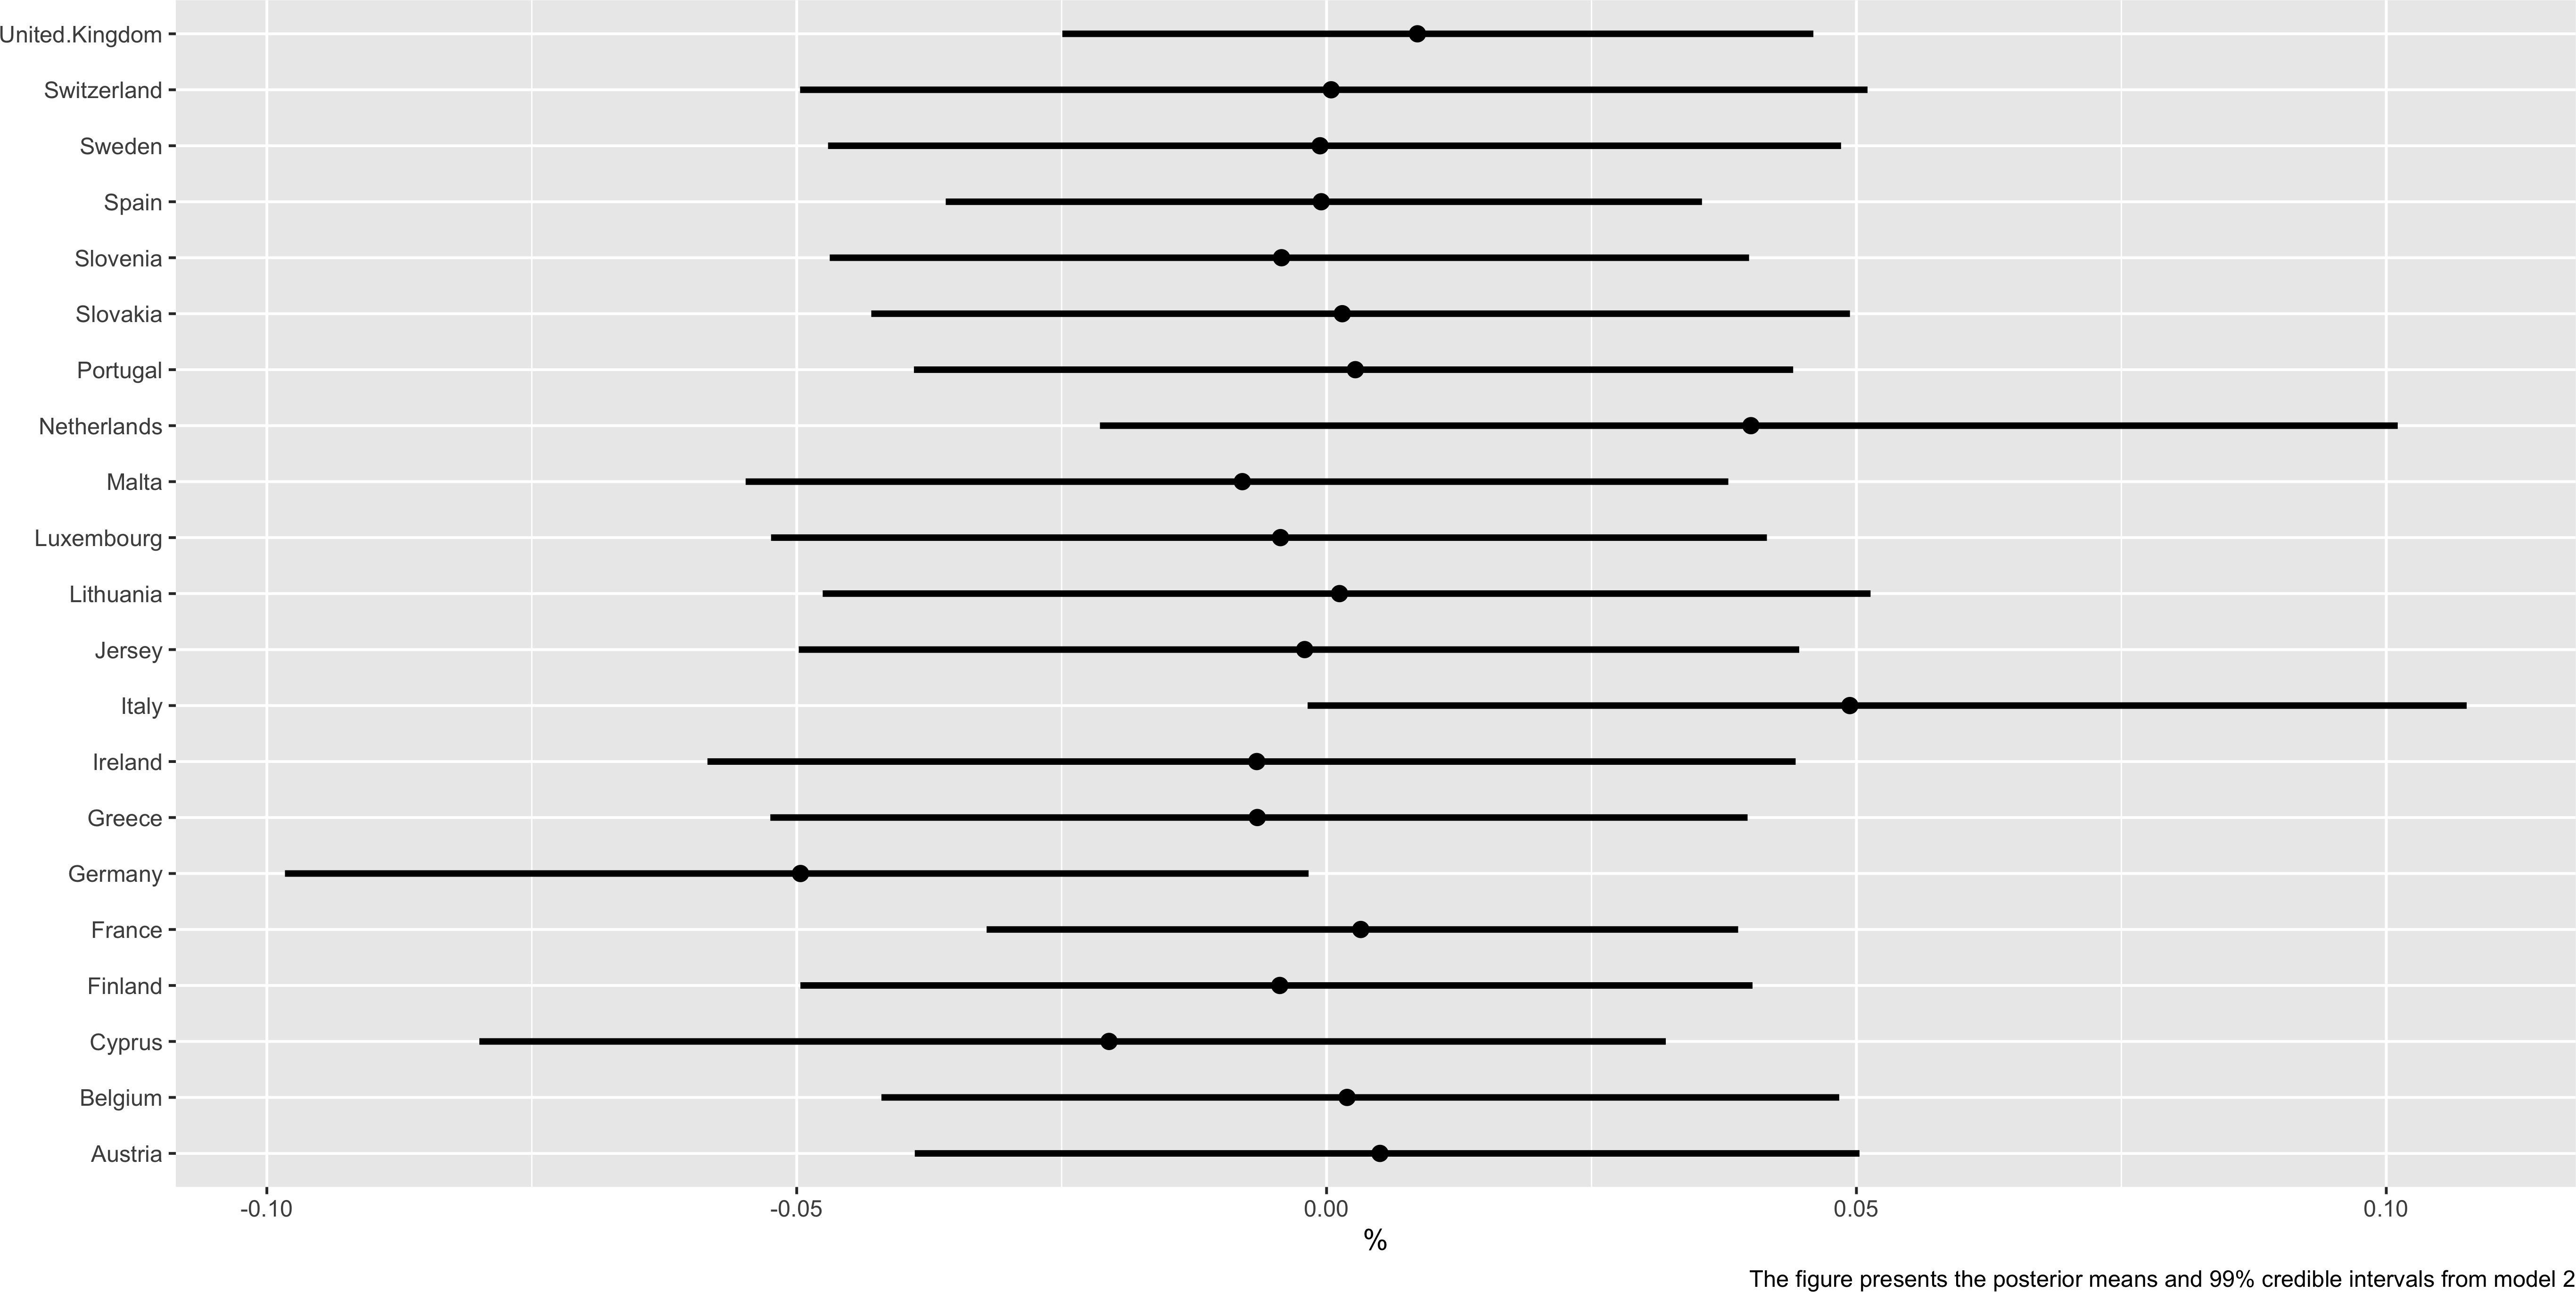
\includegraphics{figures/paper-fig7-1} \caption{Posterior probability distributions for country level random effects of ambiguous policy actions}\label{fig:fig7}
\end{figure}

Figures 4-6 disentangle the pooled effects of the baseline model into
random effects at the country level. Overall, the effect of MCR policy
actions on individual system risk is weak, with banks in many countries
showing little impact from policy actions one quarter on. Figure 4
depicts the effect of tightening actions and notably reveals that Greek,
Irish, and UK banks appear to be the driving the baseline positive
relationship. The 99\% intervals in each of these countries are
statistically meaningful. Interestingly, when we compare effect
size\footnote{Recall that the predictor variables are standardise to be
  on the same scale and thus directly comparable.} loosening actions
have the exhibit the strongest effect (-0.13 average reduction on
quarterly systemic risk for a one standard deviation move in the
predictor), although the estimate is rather noisy with a credibility
interval of {[}-0.139,0.141{]}.

\hypertarget{conclusion}{%
\section{Conclusion}\label{conclusion}}

The global financial crisis highlighted how losses at individual
financial institutions could spread across the financial system, giving
rise to systemic risk, and underscoring the importance of regulation and
supervision to a well-functioning banking system. This paper assesses
the contribution of European capital adequacy policy actions to
bank-level system-wide risk. We focus on the MaPPED database of European
policy actions. The sample offers a detailed overview of the
``life-cycle'' of policy instruments that are either genuinely
macroprudential or essentially microprudential but \emph{all} intended
to impact the banking system significantly. Our study considers the
subcategory of minimum capital requirement policy actions and use a
flexible Bayesian hierarchical model to systemic risk implications of
such actions. We enumerate our hypotheses using \(\Delta CoVaR\) within
a flexible Bayesian framework. Specifically, Maximum a Posteriori or
\(MaP\) estimates from the posterior probabilities enter a second stage
Bayesian hierarchical model depicting policy action impacts at multiple
levels.

Overall, the MCR policy actions have a weak effect on systemic risk,
with banks in many countries showing little impact from policy actions
one quarter. Notably, our results point to a positive link between the
build-up of tightening policy actions and systemic risk. Specifically
our baseline model estimates a global random effect of 0.058 with a 95\%
posterior credible interval of {[}0.011,0.105{]}. Our hierarchical model
disentangles this result, suggesting that banks in Greece, Ireland and
the UK seem to be driving this effect. Interestingly, our models allow
us to compare effect size identifying loosening policies have the
largest relative impact (-0.13 reduction in average quarter systemic
risk for a one standard deviation move in the predictor) although, this
action's estimate is quite noisy with a credibility interval of
{[}-0.139,0.141{]}.

Systemic risk can emanate from large institutions which are highly
interconnected, but importantly, several smaller institutions may be
systemic as a herd. We argue that banks tend to choose correlated risks
during periods of increasing regulatory pressure and compliance
constraints and invest in correlated assets. This choice could increase
`herding'' as bank managers must benchmark themselves to regulatory
imposed industry standards. This type of market inefficiency could
increase rather than decrease systemic risk.

\hypertarget{appendix}{%
\section{Appendix}\label{appendix}}

\hypertarget{table-a.1}{%
\subsubsection{Table A.1}\label{table-a.1}}

\begin{longtable}[]{@{}ccc@{}}
\toprule
\begin{minipage}[b]{0.36\columnwidth}\centering
Variable\strut
\end{minipage} & \begin{minipage}[b]{0.32\columnwidth}\centering
Description\strut
\end{minipage} & \begin{minipage}[b]{0.24\columnwidth}\centering
Frequency\strut
\end{minipage}\tabularnewline
\midrule
\endhead
\begin{minipage}[t]{0.36\columnwidth}\centering
Change in the three-month yield\strut
\end{minipage} & \begin{minipage}[t]{0.32\columnwidth}\centering
Measured as the Change in the three-month Bund rate\strut
\end{minipage} & \begin{minipage}[t]{0.24\columnwidth}\centering
\strut
\end{minipage}\tabularnewline
\begin{minipage}[t]{0.36\columnwidth}\centering
Change in the slope of the yield\strut
\end{minipage} & \begin{minipage}[t]{0.32\columnwidth}\centering
Measured as the Change in the spread between the long-term composite
bond and the three-month Treasury bill rate.\strut
\end{minipage} & \begin{minipage}[t]{0.24\columnwidth}\centering
\strut
\end{minipage}\tabularnewline
\begin{minipage}[t]{0.36\columnwidth}\centering
TED spread\strut
\end{minipage} & \begin{minipage}[t]{0.32\columnwidth}\centering
Measured as the difference between the three-month EURIBOR rate and the
three-month secondary market bund rate.\strut
\end{minipage} & \begin{minipage}[t]{0.24\columnwidth}\centering
Refinitiv\strut
\end{minipage}\tabularnewline
\begin{minipage}[t]{0.36\columnwidth}\centering
Change in the credit spread\strut
\end{minipage} & \begin{minipage}[t]{0.32\columnwidth}\centering
Measured as the Change in the spread between the 10-year BAA rated bonds
and the 10-year Treasury bonds.\strut
\end{minipage} & \begin{minipage}[t]{0.24\columnwidth}\centering
Refinitiv\strut
\end{minipage}\tabularnewline
\begin{minipage}[t]{0.36\columnwidth}\centering
Europe market returns\strut
\end{minipage} & \begin{minipage}[t]{0.32\columnwidth}\centering
Daily\strut
\end{minipage} & \begin{minipage}[t]{0.24\columnwidth}\centering
Refinitiv\strut
\end{minipage}\tabularnewline
\begin{minipage}[t]{0.36\columnwidth}\centering
Daily housing sector excess returns\strut
\end{minipage} & \begin{minipage}[t]{0.32\columnwidth}\centering
Daily\strut
\end{minipage} & \begin{minipage}[t]{0.24\columnwidth}\centering
Refinitiv\strut
\end{minipage}\tabularnewline
\begin{minipage}[t]{0.36\columnwidth}\centering
Equity volatility\strut
\end{minipage} & \begin{minipage}[t]{0.32\columnwidth}\centering
Which is computed as the 22-day rolling standard deviation of daily
equity market returns\strut
\end{minipage} & \begin{minipage}[t]{0.24\columnwidth}\centering
Daily\strut
\end{minipage}\tabularnewline
\bottomrule
\end{longtable}

\hypertarget{a2-casual-path-analysis-of-risk-and-prudential-policy-actions}{%
\subsubsection{A:2: Casual path analysis of risk and prudential policy
actions}\label{a2-casual-path-analysis-of-risk-and-prudential-policy-actions}}

Causal inference requires the analyst to stop coding and start thinking
about the prior knowledge that guides the theoretical (unobserved)
causal mechanism. The fragility of inference without theory has long
been hammered home by economists (Wolpin 2014). In recent yearly, a
mathematical graph schema, well-established in social science (Elwert
and Winship 2014), is filtering into modern econometric practice.
Building on early work Wright (1934), Pearl (2009) formalised a
\emph{mathematics of causal relations}(Pearl 2010) with a central role
given to the tractable directed acyclic graphs (DAG).

DAGs are excellent teaching tools for casual inference given their
intuitive and non-technical nature (Cunningham 2021). Put simply, DAGs
encode the researcher's qualitative causal assumption about the data
generating process abstracted from sampling variability (Elwert and
Winship 2014). Casual effects can happen directly \(D \to Y\) or they
can be mediated by a third variable \(D \to X \to Y\)\footnote{Note that
  in this set-up D represents the treatment of exposure (e.g a policy
  action), Y represent outcome of interest (e,g, systemic risk) and X
  could be observable bank-level characteristics that affect both policy
  action implementation and systemic risk}. Analogous to econometric
identification, a DAG should represent the state-of-the-art
knowledge\footnote{This includes but is not limited to economic theory,
  experience, literature reviews, as well as the developed intuitions of
  the analyst} about the phenomena under investigation (Cunningham
2021).

\begin{figure}[H]
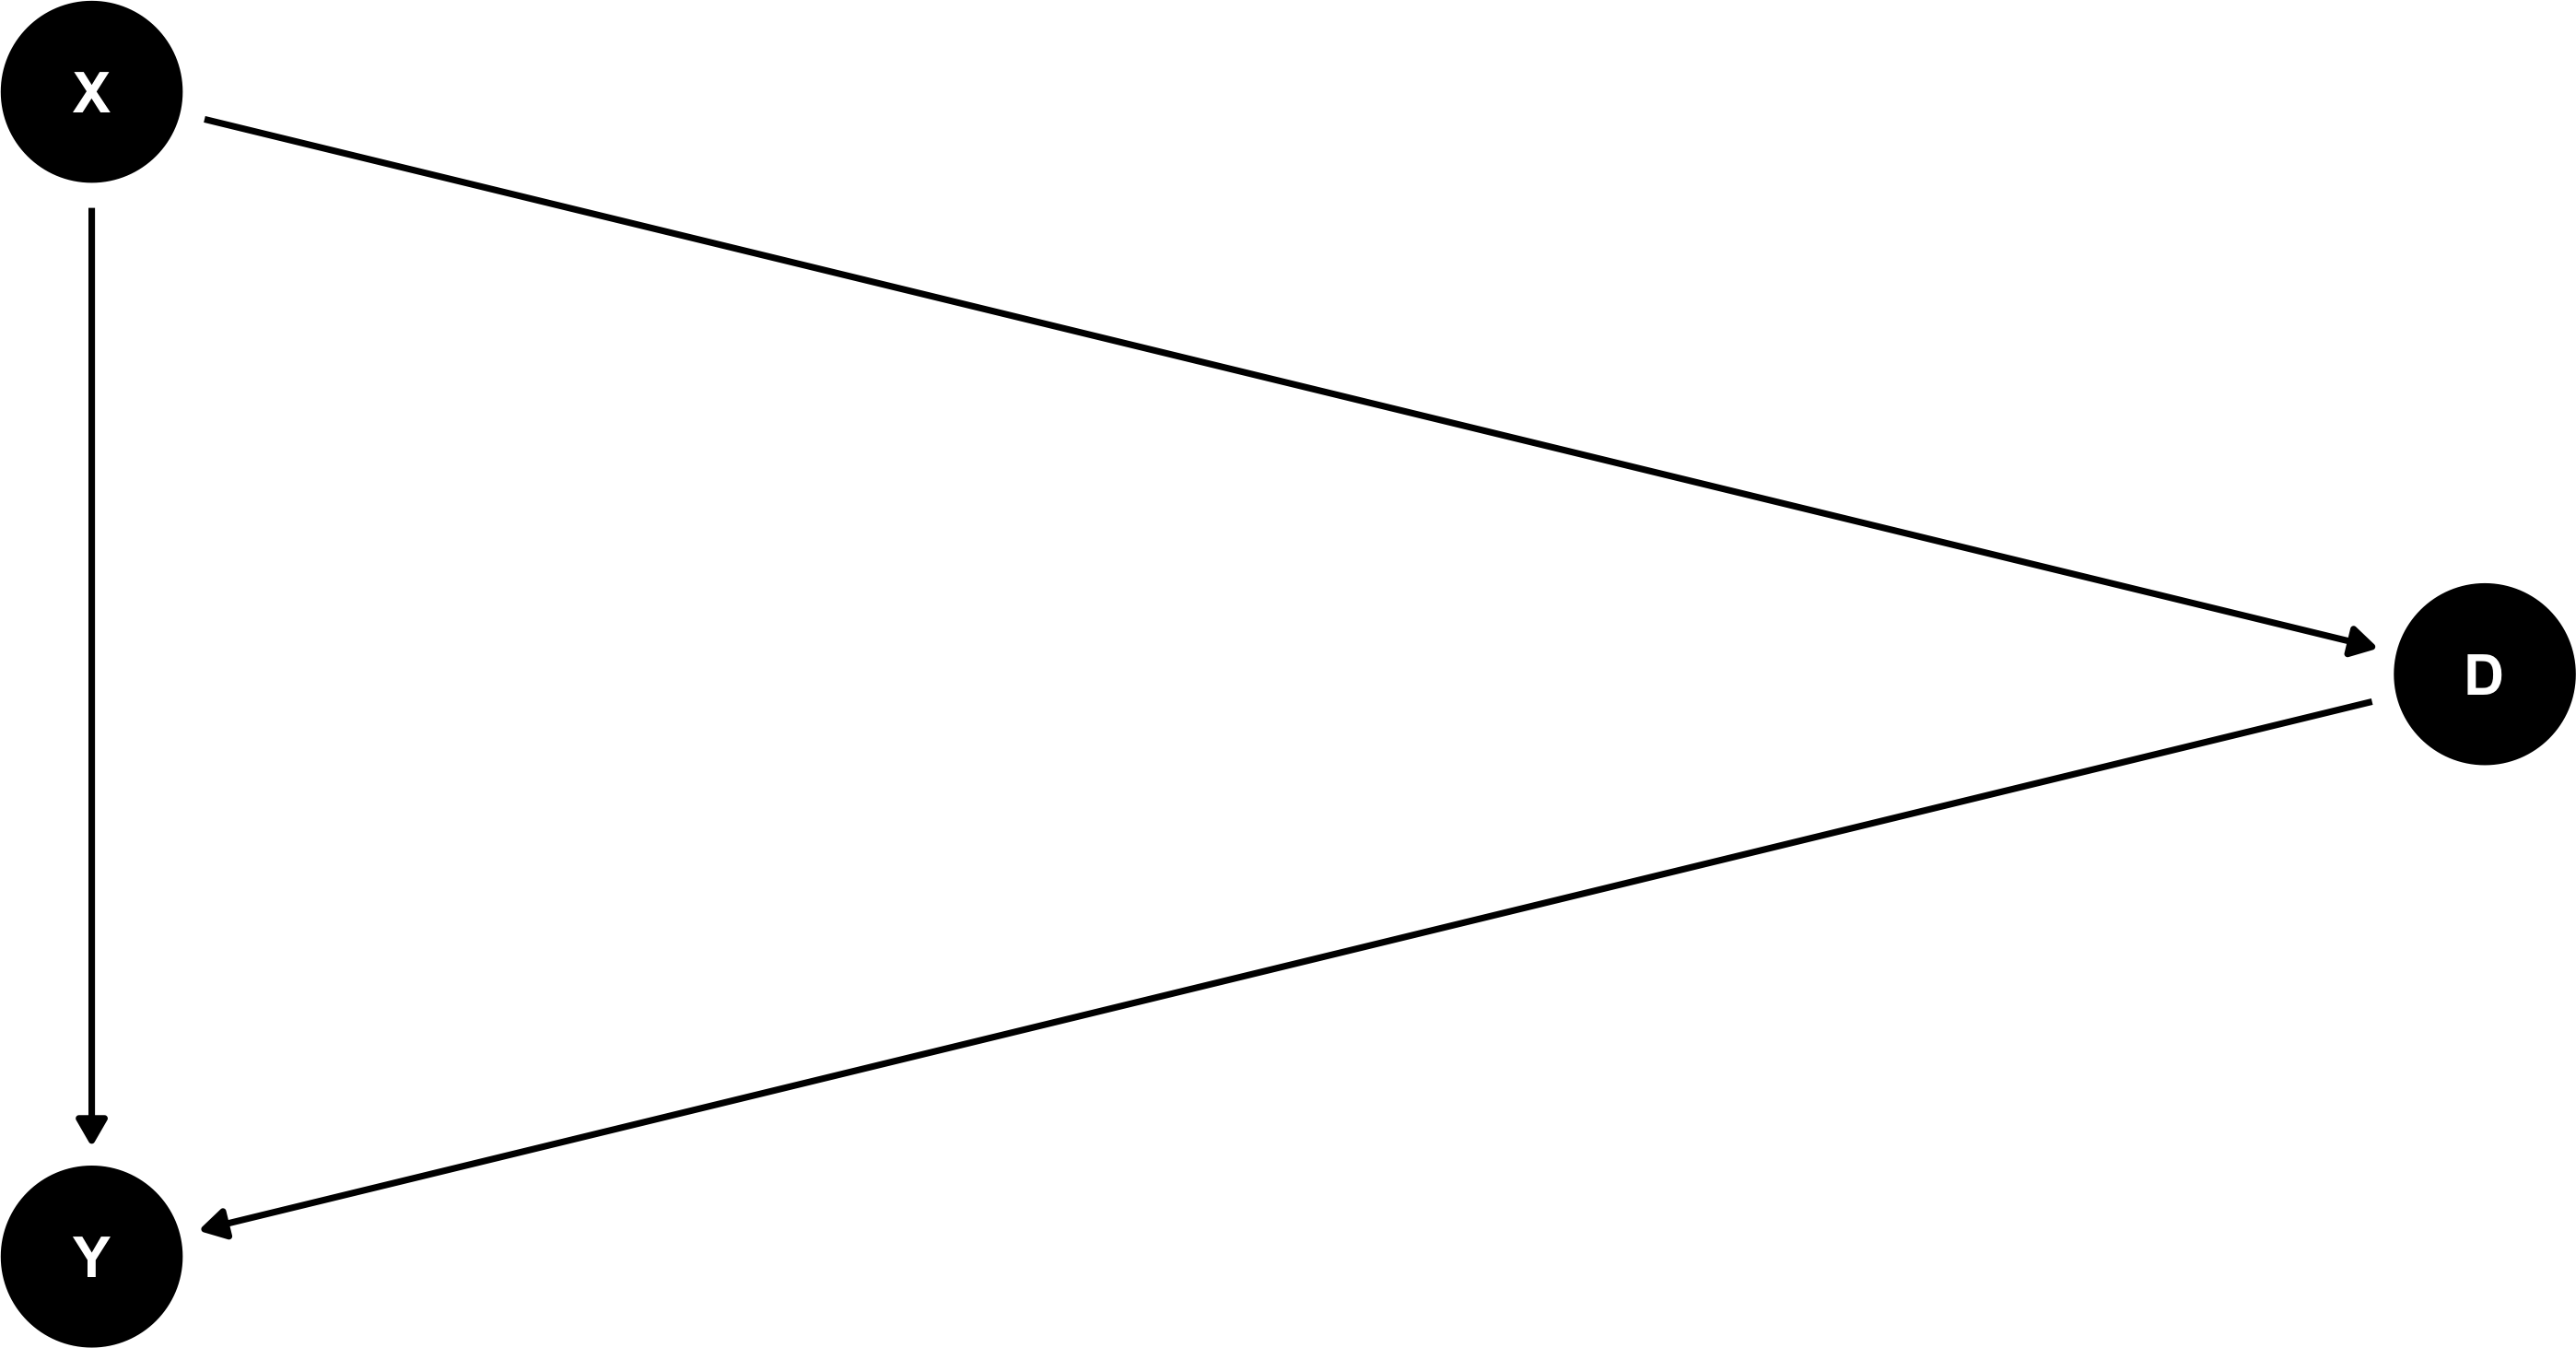
\includegraphics{figures/paper-unnamed-chunk-2-1} \caption{Confounding causal path}\label{fig:unnamed-chunk-2}
\end{figure}

Consider this hypothetical example in Figure 7, which should three
random variables with directed causal pathways Y, D and X.In DAGs
parlance, to identify an unbiased casual effect of the exposure (D) on
the outcome (Y), we must close all non-casual (or backdoor paths). In
the above graph there are two paths \(D \rightarrow Y\) and
\(D \leftarrow X \rightarrow Y\) the backdoor path. X can be thought of
as a confounding variable, fluctuations in X cause a spurious
relationship from D to Y. Thus to identify the unbiased causal
relationship of interest we close this path by controlling for X. An
example of this bias in econometrics is omitted variable bias, which can
be eliminated with common identification strategies such as instrumental
variables or diff-in-diff.

\begin{figure}[H]
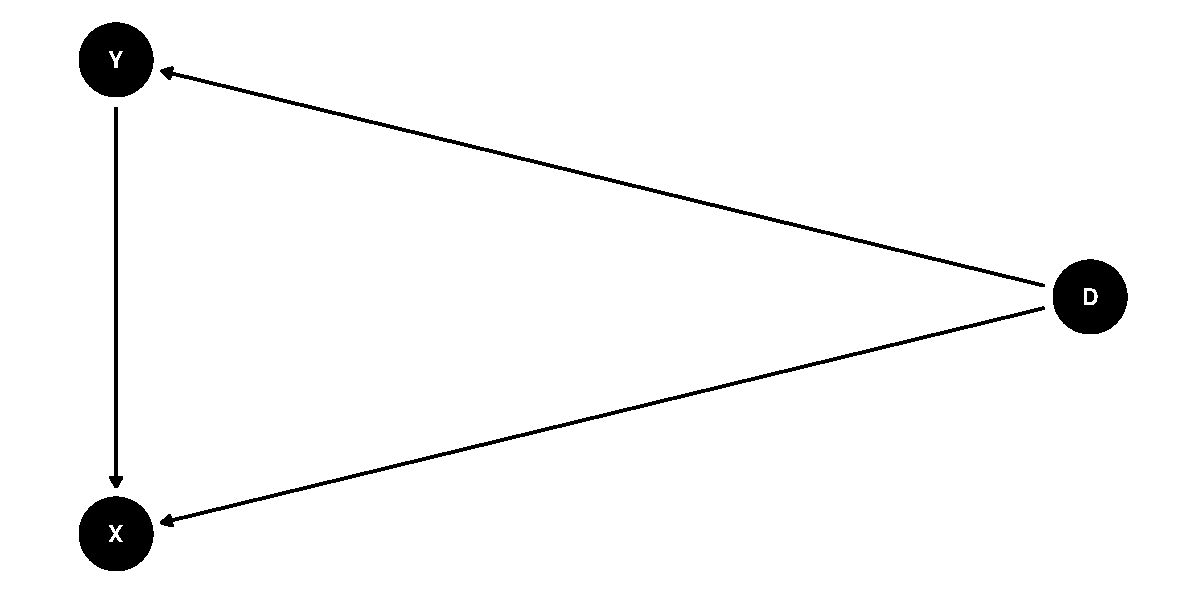
\includegraphics{figures/paper-unnamed-chunk-3-1} \caption{Confounding causal path}\label{fig:unnamed-chunk-3}
\end{figure}

The previous example is intuitively easy to understand, but the collider
variable is more subtle and challenging to grasp. Figure 8 provides an
illustration an example of a collider variable \(X\). There are now two
paths \(D \rightarrow Y\) and \(D \rightarrow X \leftarrow Y\) the
backdoor path. Specifically, the casual effects of Y and D collide at X,
naturally closing non-causal path. Collider variables, unlike
confounders, naturally close non-causal paths and the mistake that can
be made is that if we control for these variables this opens a
non-causal path inducing bias. Collider bias is also known as endogenous
selection bias and is far less intuitive and straightforward than
confounding bias.

\begin{figure}[H]
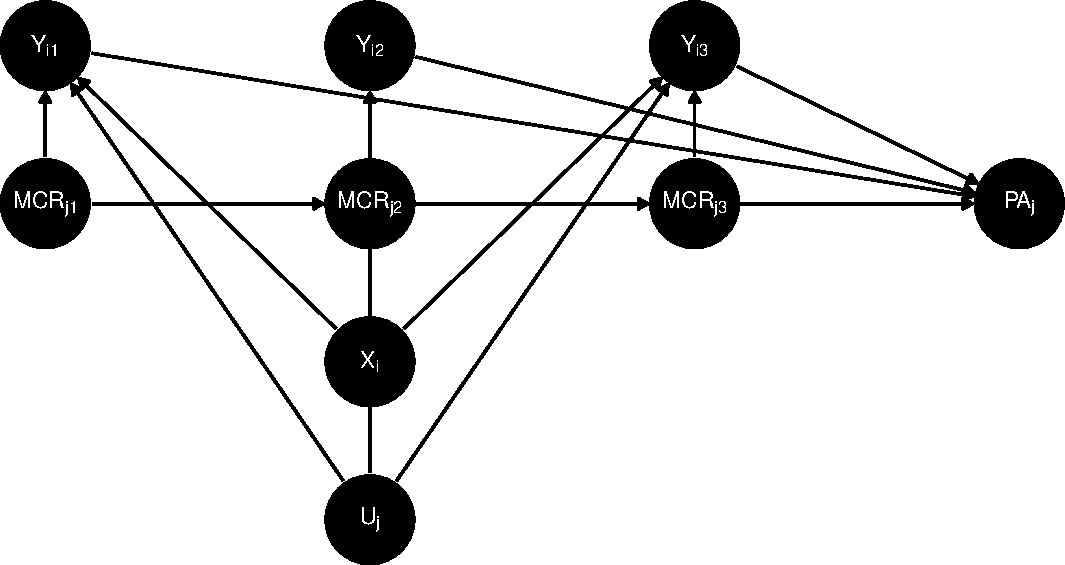
\includegraphics{figures/paper-panel_dag-1} \caption{Hierarchical casual mechanism}\label{fig:panel_dag}
\end{figure}

Figure 9 illustrates a more complex DAG relating our phenomenon of
interest. The figure represents causal relationship between minimum
capital requirements (\(MCR_j\)) actions, other policy actions
(\(PA_j\)), bank-level covariates (\(X_i\)), latent country effects
(\(Uj\)) and systemic risk \(Y_i\) for \(t=1,2,3\). This DAG is adapted
from the unit fixed effects graph in Imai and Kim (2019). In the
language of DAGs, \(PA_j\) is a collider variable affected by
fluctuations in \(MCR_{jt}\) and \(Y_{it}\). This suggests that
including other policy actions in a regression specification would
induce bias in the analysis by opening this non-causal path.

There is some merit to this theoretical argument in the data. In the
MaPPeD data there are many other prudential policy actions that are
themselves effects by the MCR actions and the levels of systemic risk.
For example, there are 192 policy actions which are identified as having
the potential for reciprocity to counteract cross-border lending
activities. Cantone, Jahn, and Rancoita (2019) shows that the
application of cross-border reciprocity arrangements would reduce the
need for capital requirements needed to achieve the same goal. This
effectively shows that such reciprocity arrangement in other prudential
policies, such as countercyclical capital buffers, has a direct causal
path to capital requirements. Clearly, the level of systemic risk will
also affect the amount of other policy actions imposed.

\hypertarget{references}{%
\section{References}\label{references}}

\setlength{\parindent}{-0.2in}
\setlength{\leftskip}{0.2in}
\setlength{\parskip}{8pt}
\vspace*{-0.2in}

\noindent

\hypertarget{refs}{}
\leavevmode\hypertarget{ref-Acharya2009}{}%
Acharya, Viral V. 2009. ``A Theory of Systemic Risk and Design of
Prudential Bank Regulation.'' \emph{Journal of Financial Stability} 5
(3): 224--55.

\leavevmode\hypertarget{ref-Acharya2007}{}%
Acharya, Viral V, and Tanju Yorulmazer. 2007. ``Too Many to Fail---an
Analysis of Time-Inconsistency in Bank Closure Policies.'' \emph{Journal
of Financial Intermediation} 16 (1): 1--31.

\leavevmode\hypertarget{ref-Adrian2016}{}%
Adrian, Tobias, and Markus K Brunnermeier. 2016. ``CoVaR.'' \emph{Am.
Econ. Rev.} 106 (7): 1705--41.

\leavevmode\hypertarget{ref-Agoraki2011}{}%
Agoraki, Maria-Eleni K, Manthos D Delis, and Fotios Pasiouras. 2011.
``Regulations, Competition and Bank Risk-Taking in Transition
Countries.'' \emph{Journal of Financial Stability} 7 (1): 38--48.

\leavevmode\hypertarget{ref-Akinci2017}{}%
Akinci, Ozge, and Jane Olmstead-Rumsey. 2017. ``How Effective Are
Macroprudential Policies? An Empirical Investigation.'' \emph{Journal of
Financial Intermediation}, April.

\leavevmode\hypertarget{ref-Allen2012}{}%
Allen, Franklin, Ana Babus, and Elena Carletti. 2012. ``Asset
Commonality, Debt Maturity and Systemic Risk.'' \emph{J. Financ. Econ.}
104 (3): 519--34.

\leavevmode\hypertarget{ref-angrist2008mostly}{}%
Angrist, Joshua D, and Jörn-Steffen Pischke. 2008. \emph{Mostly Harmless
Econometrics: An Empiricist's Companion}. Princeton university press.

\leavevmode\hypertarget{ref-angrist2010credibility}{}%
---------. 2010. ``The Credibility Revolution in Empirical Economics:
How Better Research Design Is Taking the Con Out of Econometrics.''
\emph{Journal of Economic Perspectives} 24 (2): 3--30.

\leavevmode\hypertarget{ref-Ayadi2020}{}%
Ayadi, Rym, Paola Bongini, Barbara Casu, and Doriana Cucinelli. 2020.
``Bank Business Model Migrations in Europe: Determinants and Effects.''
\emph{Br. J. Manag.}, nos. 1467-8551.12437 (November).

\leavevmode\hypertarget{ref-Barth2001}{}%
Barth, James, Gerard Caprio, and Ross Levine. 2001. ``Bank Regulation
and Supervision: A New Database.'' \emph{Brookings-Wharton Papers on
Financial Services}.

\leavevmode\hypertarget{ref-Barth2004}{}%
Barth, James R, Gerard Caprio Jr., and Ross Levine. 2004. ``Bank
Regulation and Supervision: What Works Best?'' \emph{Journal of
Financial Intermediation} 13 (2): 205--48.

\leavevmode\hypertarget{ref-Barth2006}{}%
Barth, James R, Gerard Caprio, and Ross Levine. 2006. \emph{Rethinking
Bank Regulation: Till Angels Govern}. Edited by Govern, Till, and
Angels. Second edi. New York: Cambridge University Press.

\leavevmode\hypertarget{ref-Barth2008}{}%
---------. 2008. ``Bank Regulations Are Changing: For Better or Worse?''
\emph{Comp. Econ. Stud.} 50 (4): 537--63.

\leavevmode\hypertarget{ref-Barth2012}{}%
---------. 2012. \emph{Guardians of Finance: Making Regulators Work for
Us}. MIT Press.

\leavevmode\hypertarget{ref-Behn2016}{}%
Behn, Markus, Rainer F H Haselmann, and Vikrant Vig. 2016. ``The Limits
of Model-Based Regulation,'' July.

\leavevmode\hypertarget{ref-Bernardi2013}{}%
Bernardi, Mauro, Ghislaine Gayraud, and Lea Petrella. 2013. ``Bayesian
Inference for CoVaR,'' June. \url{http://arxiv.org/abs/1306.2834}.

\leavevmode\hypertarget{ref-Brunnermeier2020}{}%
Brunnermeier, Markus, Simon Rother, and Isabel Schnabel. 2020. ``Asset
Price Bubbles and Systemic Risk.'' \emph{Rev. Financ. Stud.} 33 (9):
4272--4317.

\leavevmode\hypertarget{ref-Budnik2018}{}%
Budnik, Katarzyna Barbara, and Johannes Kleibl. 2018. ``Macroprudential
Regulation in the European Union in 1995-2014: Introducing a New Data
Set on Policy Actions of a Macroprudential Nature.'' \emph{European
Central Bank Working Paper Series}, no. 2123 (January).

\leavevmode\hypertarget{ref-Cantone2019}{}%
Cantone, David, Nadya Jahn, and Elena Rancoita. 2019. ``Thinking Beyond
Borders: How Important Are Reciprocity Arrangements for the Use of
Sectoral Capital Buffers.'' European Central Bank.

\leavevmode\hypertarget{ref-Carroll2006}{}%
Carroll, Raymond J, David Ruppert, Leonard A Stefanski, and Ciprian M
Crainiceanu. 2006. \emph{Measurement Error in Nonlinear Models: A Modern
Perspective, Second Edition}. CRC Press.

\leavevmode\hypertarget{ref-Cerutti2017}{}%
Cerutti, Eugenio, Stijn Claessens, and Luc Laeven. 2017. ``The Use and
Effectiveness of Macroprudential Policies: New Evidence.'' \emph{Journal
of Financial Stability} 28 (February): 203--24.

\leavevmode\hypertarget{ref-Cerutti2016}{}%
Cerutti, Mr Eugenio M, Mr Ricardo Correa, Elisabetta Fiorentino, and
Esther Segalla. 2016. \emph{Changes in Prudential Policy Instruments ---
a New Cross-Country Database}. International Monetary Fund.

\leavevmode\hypertarget{ref-Cunningham2021}{}%
Cunningham, Scott. 2021. \emph{Causal Inference: The Mixtape}. Yale
University Press.

\leavevmode\hypertarget{ref-Danielsson2012}{}%
Danielsson, Jon, Hyun Song Shin, and Jean-Pierre Zigrand. 2012.
``Endogenous and Systemic Risk.'' In \emph{Quantifying Systemic Risk},
73--94. University of Chicago Press.

\leavevmode\hypertarget{ref-Delis2011}{}%
Delis, Manthos D, and Panagiotis K Staikouras. 2011. ``Supervisory
Effectiveness and Bank Risk.'' \emph{Rev Financ} 15 (3): 511--43.

\leavevmode\hypertarget{ref-Demirguc-Kunt2011}{}%
Demirgüç-Kunt, Asli, and Enrica Detragiache. 2011. ``Basel Core
Principles and Bank Soundness: Does Compliance Matter?'' \emph{Journal
of Financial Stability} 7 (4): 179--90.

\leavevmode\hypertarget{ref-Elwert2014}{}%
Elwert, Felix, and Christopher Winship. 2014. ``Endogenous Selection
Bias: The Problem of Conditioning on a Collider Variable.'' \emph{Annu.
Rev. Sociol.} 40 (July): 31--53.

\leavevmode\hypertarget{ref-Embrechts2001}{}%
Embrechts, Paul, Jon Danielsson, Charles A E Goodhart, Con Keating,
Felix Muennich, Olivier Renault, and Hyun Song Shin. 2001. ``An Academic
Response to Basel II.'' \emph{FMG Special Paper 130} 130.

\leavevmode\hypertarget{ref-Fan2020}{}%
Fan, Jianqing, Yuan Ke, and Kaizheng Wang. 2020. ``Factor-Adjusted
Regularized Model Selection.'' \emph{J. Econom.} 216 (1): 71--85.

\leavevmode\hypertarget{ref-Farhi2012}{}%
Farhi, Emmanuel, and Jean Tirole. 2012. ``Collective Moral Hazard,
Maturity Mismatch, and Systemic Bailouts.'' \emph{Am. Econ. Rev.} 102
(1): 60--93.

\leavevmode\hypertarget{ref-Gehrig2017}{}%
Gehrig, Thomas, and Maria Chiara Iannino. 2017. ``Did the Basel Process
of Capital Regulation Enhance the Resiliency of European Banks?''
\emph{CEPR Discussion Paper No. DP11920}.

\leavevmode\hypertarget{ref-Gelman2013}{}%
Gelman, Andrew, John B Carlin, Hal S Stern, David B Dunson, Aki Vehtari,
and Donald B Rubin. 2013. \emph{Bayesian Data Analysis, Third Edition}.
CRC Press.

\leavevmode\hypertarget{ref-Gelman2019}{}%
Gelman, Andrew, Ben Goodrich, Jonah Gabry, and Aki Vehtari. 2019.
``R-Squared for Bayesian Regression Models.'' \emph{Am. Stat.} 73 (3):
307--9.

\leavevmode\hypertarget{ref-Gelman2007}{}%
Gelman, Andrew, and Jennifer Hill. 2007. \emph{Data Analysis Using
Regression and Multilevel/Hierarchical Models}. Cambridge University
Press.

\leavevmode\hypertarget{ref-Greene2014}{}%
Greene, William H. 2014. \emph{Econometric Analysis: International
Edition: Global Edition}. Pearson Higher Ed.

\leavevmode\hypertarget{ref-Hirakata2017}{}%
Hirakata, Naohisa, Yosuke Kido, and Jie Liang Thum. 2017. ``Empirical
Evidence on `Systemic as a Herd': The Case of Japanese Regional Banks.''
\emph{Bank of Japan Working Paper Series}.

\leavevmode\hypertarget{ref-Horvath2017}{}%
Horváth, Bálint L, and Wolf Wagner. 2017. ``The Disturbing Interaction
Between Countercyclical Capital Requirements and Systemic Risk.''
\emph{Rev Financ} 21 (4): 1485--1511.

\leavevmode\hypertarget{ref-Hsiao2014}{}%
Hsiao, Cheng. 2014. \emph{Analysis of Panel Data}. Cambridge University
Press.

\leavevmode\hypertarget{ref-Imai2019}{}%
Imai, Kosuke, and In Song Kim. 2019. ``When Should We Use Unit Fixed
Effects Regression Models for Causal Inference with Longitudinal Data?''
\emph{Am. J. Pol. Sci.} 63 (2): 467--90.

\leavevmode\hypertarget{ref-Klomp2012}{}%
Klomp, Jeroen, and Jakob de Haan. 2012. ``Banking Risk and Regulation:
Does One Size Fit All?'' \emph{Journal of Banking \& Finance} 36 (12):
3197--3212.

\leavevmode\hypertarget{ref-Li2010}{}%
Li, Qing, Ruibin Xi, and Nan Lin. 2010. ``Bayesian Regularized Quantile
Regression.'' \emph{Bayesian Anal.} 5 (3): 533--56.

\leavevmode\hypertarget{ref-Lin2012}{}%
Lin, Nan, and Chao Chang. 2012. ``Comment on Article by Lum and
Gelfand.'' \emph{Bayesian Analysis}.

\leavevmode\hypertarget{ref-Meuleman2019}{}%
Meuleman, Elien, and Rudi Vander Vennet. 2019. ``Macroprudential Policy
and Bank Systemic Risk.''

\leavevmode\hypertarget{ref-Mogliani2020}{}%
Mogliani, Matteo, and Anna Simoni. 2020. ``Bayesian MIDAS Penalized
Regressions: Estimation, Selection, and Prediction.'' \emph{J. Econom.},
August.

\leavevmode\hypertarget{ref-Nagel2021}{}%
Nagel, Stefan. 2021. \emph{Machine Learning in Asset Pricing}.

\leavevmode\hypertarget{ref-Nijskens2011}{}%
Nijskens, Rob, and Wolf Wagner. 2011. ``Credit Risk Transfer Activities
and Systemic Risk: How Banks Became Less Risky Individually but Posed
Greater Risks to the Financial System at the Same Time.'' \emph{Journal
of Banking \& Finance} 35 (6): 1391--8.

\leavevmode\hypertarget{ref-Pearl2010}{}%
Pearl, Judea. 2010. ``The Mathematics of Causal Relations.''
\emph{Causality and Psychopathology: Finding the Determinants of
Disorders and Their Cures (P. Shrout, K. Keyes and K. Ornstein, Eds. ).
Oxford University Press, Corvallis, OR}, 47--65.

\leavevmode\hypertarget{ref-Pearl2009}{}%
---------. 2009. \emph{Causality}. Cambridge University Press.

\leavevmode\hypertarget{ref-Pepper2002}{}%
Pepper, John V. 2002. ``Robust Inferences from Random Clustered Samples:
An Application Using Data from the Panel Study of Income Dynamics.''
\emph{Econ. Lett.} 75 (3): 341--45.

\leavevmode\hypertarget{ref-Reed2015}{}%
Reed, William Robert. 2015. ``On the Practice of Lagging Variables to
Avoid Simultaneity.'' \emph{Oxford Bulletin of Economics and
Statistics}.

\leavevmode\hypertarget{ref-Schmidt-Catran2015}{}%
Schmidt-Catran, Alexander W, and Malcolm Fairbrother. 2015. ``The Random
Effects in Multilevel Models: Getting Them Wrong and Getting Them
Right.'' \emph{Eur. Sociol. Rev.} 32 (1): 23--38.

\leavevmode\hypertarget{ref-Schneider2020}{}%
Schneider, Eric B. 2020. ``Collider Bias in Economic History Research.''
\emph{Explor. Econ. Hist.} 78 (October): 101356.

\leavevmode\hypertarget{ref-Segura2011}{}%
Segura, Anatoli, and Javier Suarez. 2011. ``Liquidity Shocks, Roll-over
Risk and Debt Maturity.'' \emph{CEPR Discussion Paper No. DP8324},
April.

\leavevmode\hypertarget{ref-Sims2010}{}%
Sims, Christopher A. 2010. ``But Economics Is Not an Experimental
Science.'' \emph{J. Econ. Perspect.} 24 (2): 59--68.

\leavevmode\hypertarget{ref-Stein2012}{}%
Stein, Jeremy C. 2012. ``Monetary Policy as Financial Stability
Regulation.'' \emph{Q. J. Econ.} 127 (1): 57--95.

\leavevmode\hypertarget{ref-Strauss2020}{}%
Strauss, Ilan, and Jangho Yang. 2020. ``Corporate Secular Stagnation:
Empirical Evidence on the Advanced Economy Investment Slowdown.''
\emph{INET Oxford Working Paper No. 2019-16}.

\leavevmode\hypertarget{ref-Tibshirani2011}{}%
Tibshirani, Robert. 2011. ``Regression Shrinkage and Selection via the
Lasso: A Retrospective.'' \emph{J. R. Stat. Soc. Series B Stat.
Methodol.} 73 (3): 273--82.

\leavevmode\hypertarget{ref-Tsionas2003}{}%
Tsionas, Efthymios G. 2003. ``Bayesian Quantile Inference.'' \emph{J.
Stat. Comput. Simul.} 73 (9): 659--74.

\leavevmode\hypertarget{ref-Vives2014}{}%
Vives, Xavier. 2014. ``Strategic Complementarity, Fragility, and
Regulation.'' \emph{Rev. Financ. Stud.} 27 (12): 3547--92.

\leavevmode\hypertarget{ref-Wolpin2014}{}%
Wolpin, Kenneth. 2014. \emph{The Limits of Inference Without Theory}.
Edited by MIT press. MIT Press.

\leavevmode\hypertarget{ref-Wooldridge2010}{}%
Wooldridge, Jeffrey M. 2010. \emph{Econometric Analysis of Cross Section
and Panel Data, Second Edition}. MIT Press.

\leavevmode\hypertarget{ref-Wooldridge2015}{}%
---------. 2015. \emph{Introductory Econometrics: A Modern Approach}.
Cengage Learning.

\leavevmode\hypertarget{ref-Wooldridge2019}{}%
---------. 2019. ``Correlated Random Effects Models with Unbalanced
Panels.'' \emph{J. Econom.} 211 (1): 137--50.

\leavevmode\hypertarget{ref-Wright1934}{}%
Wright, Sewall. 1934. ``The Method of Path Coefficients.'' \emph{Aoms} 5
(3): 161--215.

\end{document}
